\documentclass[uplatex,dvipdfmx,titlepage]{jsarticle}
\usepackage[dvipdfmx]{graphicx}
\usepackage{amsmath,amssymb}
\usepackage{bm}
\usepackage{enumitem} 
\usepackage{float}

\title{固体力学の実験}
\author{京都大学工学部物理工学科 1025363386 伊藤温大}
\date{\today}

\begin{document}
\maketitle
\tableofcontents
\clearpage

\section{はじめに}
本レポートでは、固体力学に関する光弾性法による応力場の可視化と応力集中係数の評価について、その結果および実験課題について報告する。

\section{光弾性法による応力場の可視化と応力集中係数の評価}

\subsection{目的}
曲げ応力を受ける梁の干渉縞の測定を行い、切り欠き部における応力集中係数を評価する。それによって光弾性法の原理を理解する。

\subsection{実験方法}
以下の手順で測定を行った。

\subsubsection*{課題1:基準試験片の光弾性画像と縞次数の解析}
切り欠きの無い基準試験片に対して錘の質量、支点位置、視野の明暗を調節し、光弾性画像を撮影することで縞次数を解析した。\\
実験に際して以下の器具を使用した。図\ref{fig:specimen}に示すような、ポリカーボネート製の梁を試験片として使用した。\\
図の上から順に、切り欠きなし、切り欠きの半径$\rho=1, 2, 4, 8$ mmである。
\begin{figure}[H]
    \centering
    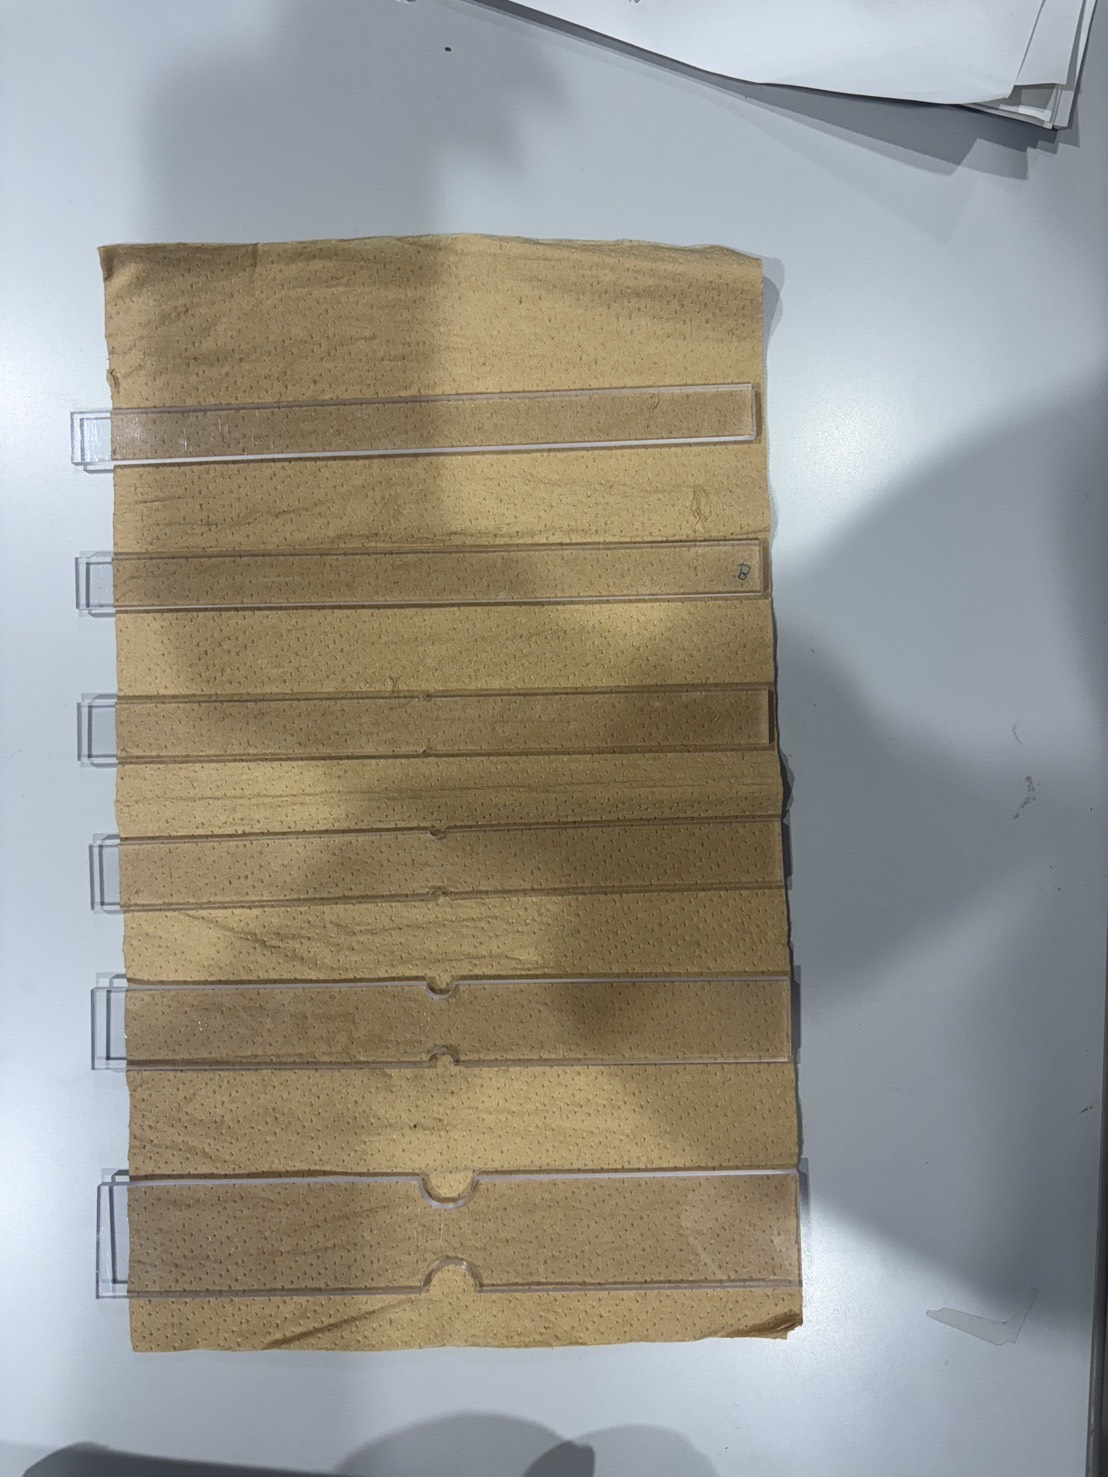
\includegraphics[height=6cm]{実験試験片.jpg}
    \caption{試験片（上から切り欠きなし、切り欠きの半径$\rho=1, 2, 4, 8$ mm）}
    \label{fig:specimen}
\end{figure}
また、図\ref{fig:bending_machine}の左にある曲げ試験装置を用いて4点曲げ試験を行った。この装置では直径10 mmのピン4本で試験片を支持し、上部から錘をのせることで荷重を作用させる。このとき錘の質量を$W$ (kg)、支点位置を$e$ (cm)として$W, e$を変化させ、実験を行った。\\
実験で使用した光学系は以下のとおりである。
\begin{enumerate}[label=\arabic*.]
    \item He-Ne レーザー
    \item レーザービームエキスパンダ
    \item 平凹レンズ
    \item 平凸レンズ
    \item CMOSカメラ
\end{enumerate}
これらの全体像は以下のようである。
\begin{figure}[H]
    \centering
    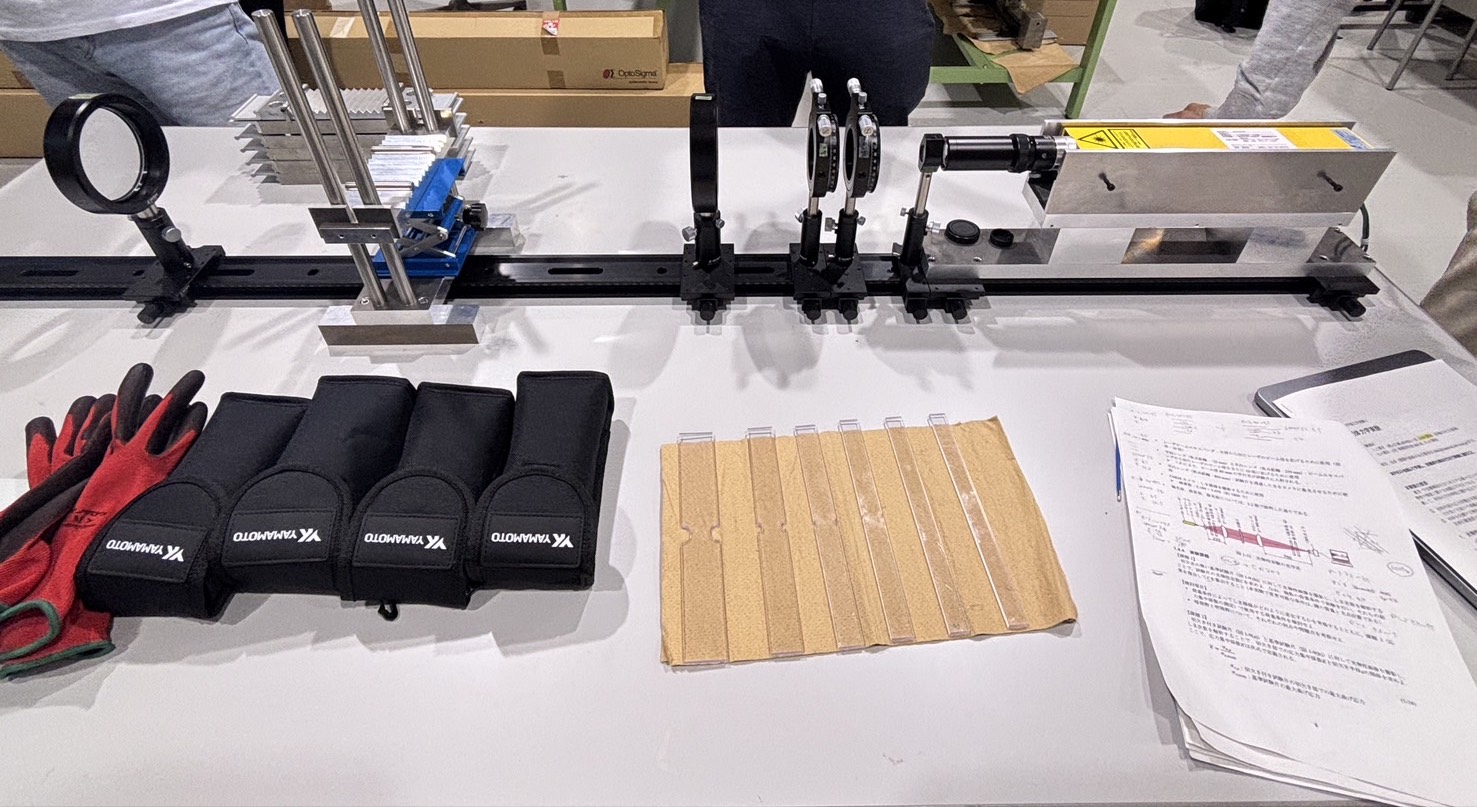
\includegraphics[width=12cm]{実験全体写真2.jpg}
    \caption{4点曲げ試験装置の概略図}
    \label{fig:bending_machine}
\end{figure}
以下が実際の実験における光弾性画像である。

\begin{figure}[H]
    \centering
    \begin{minipage}[b]{0.48\textwidth}
        \centering
        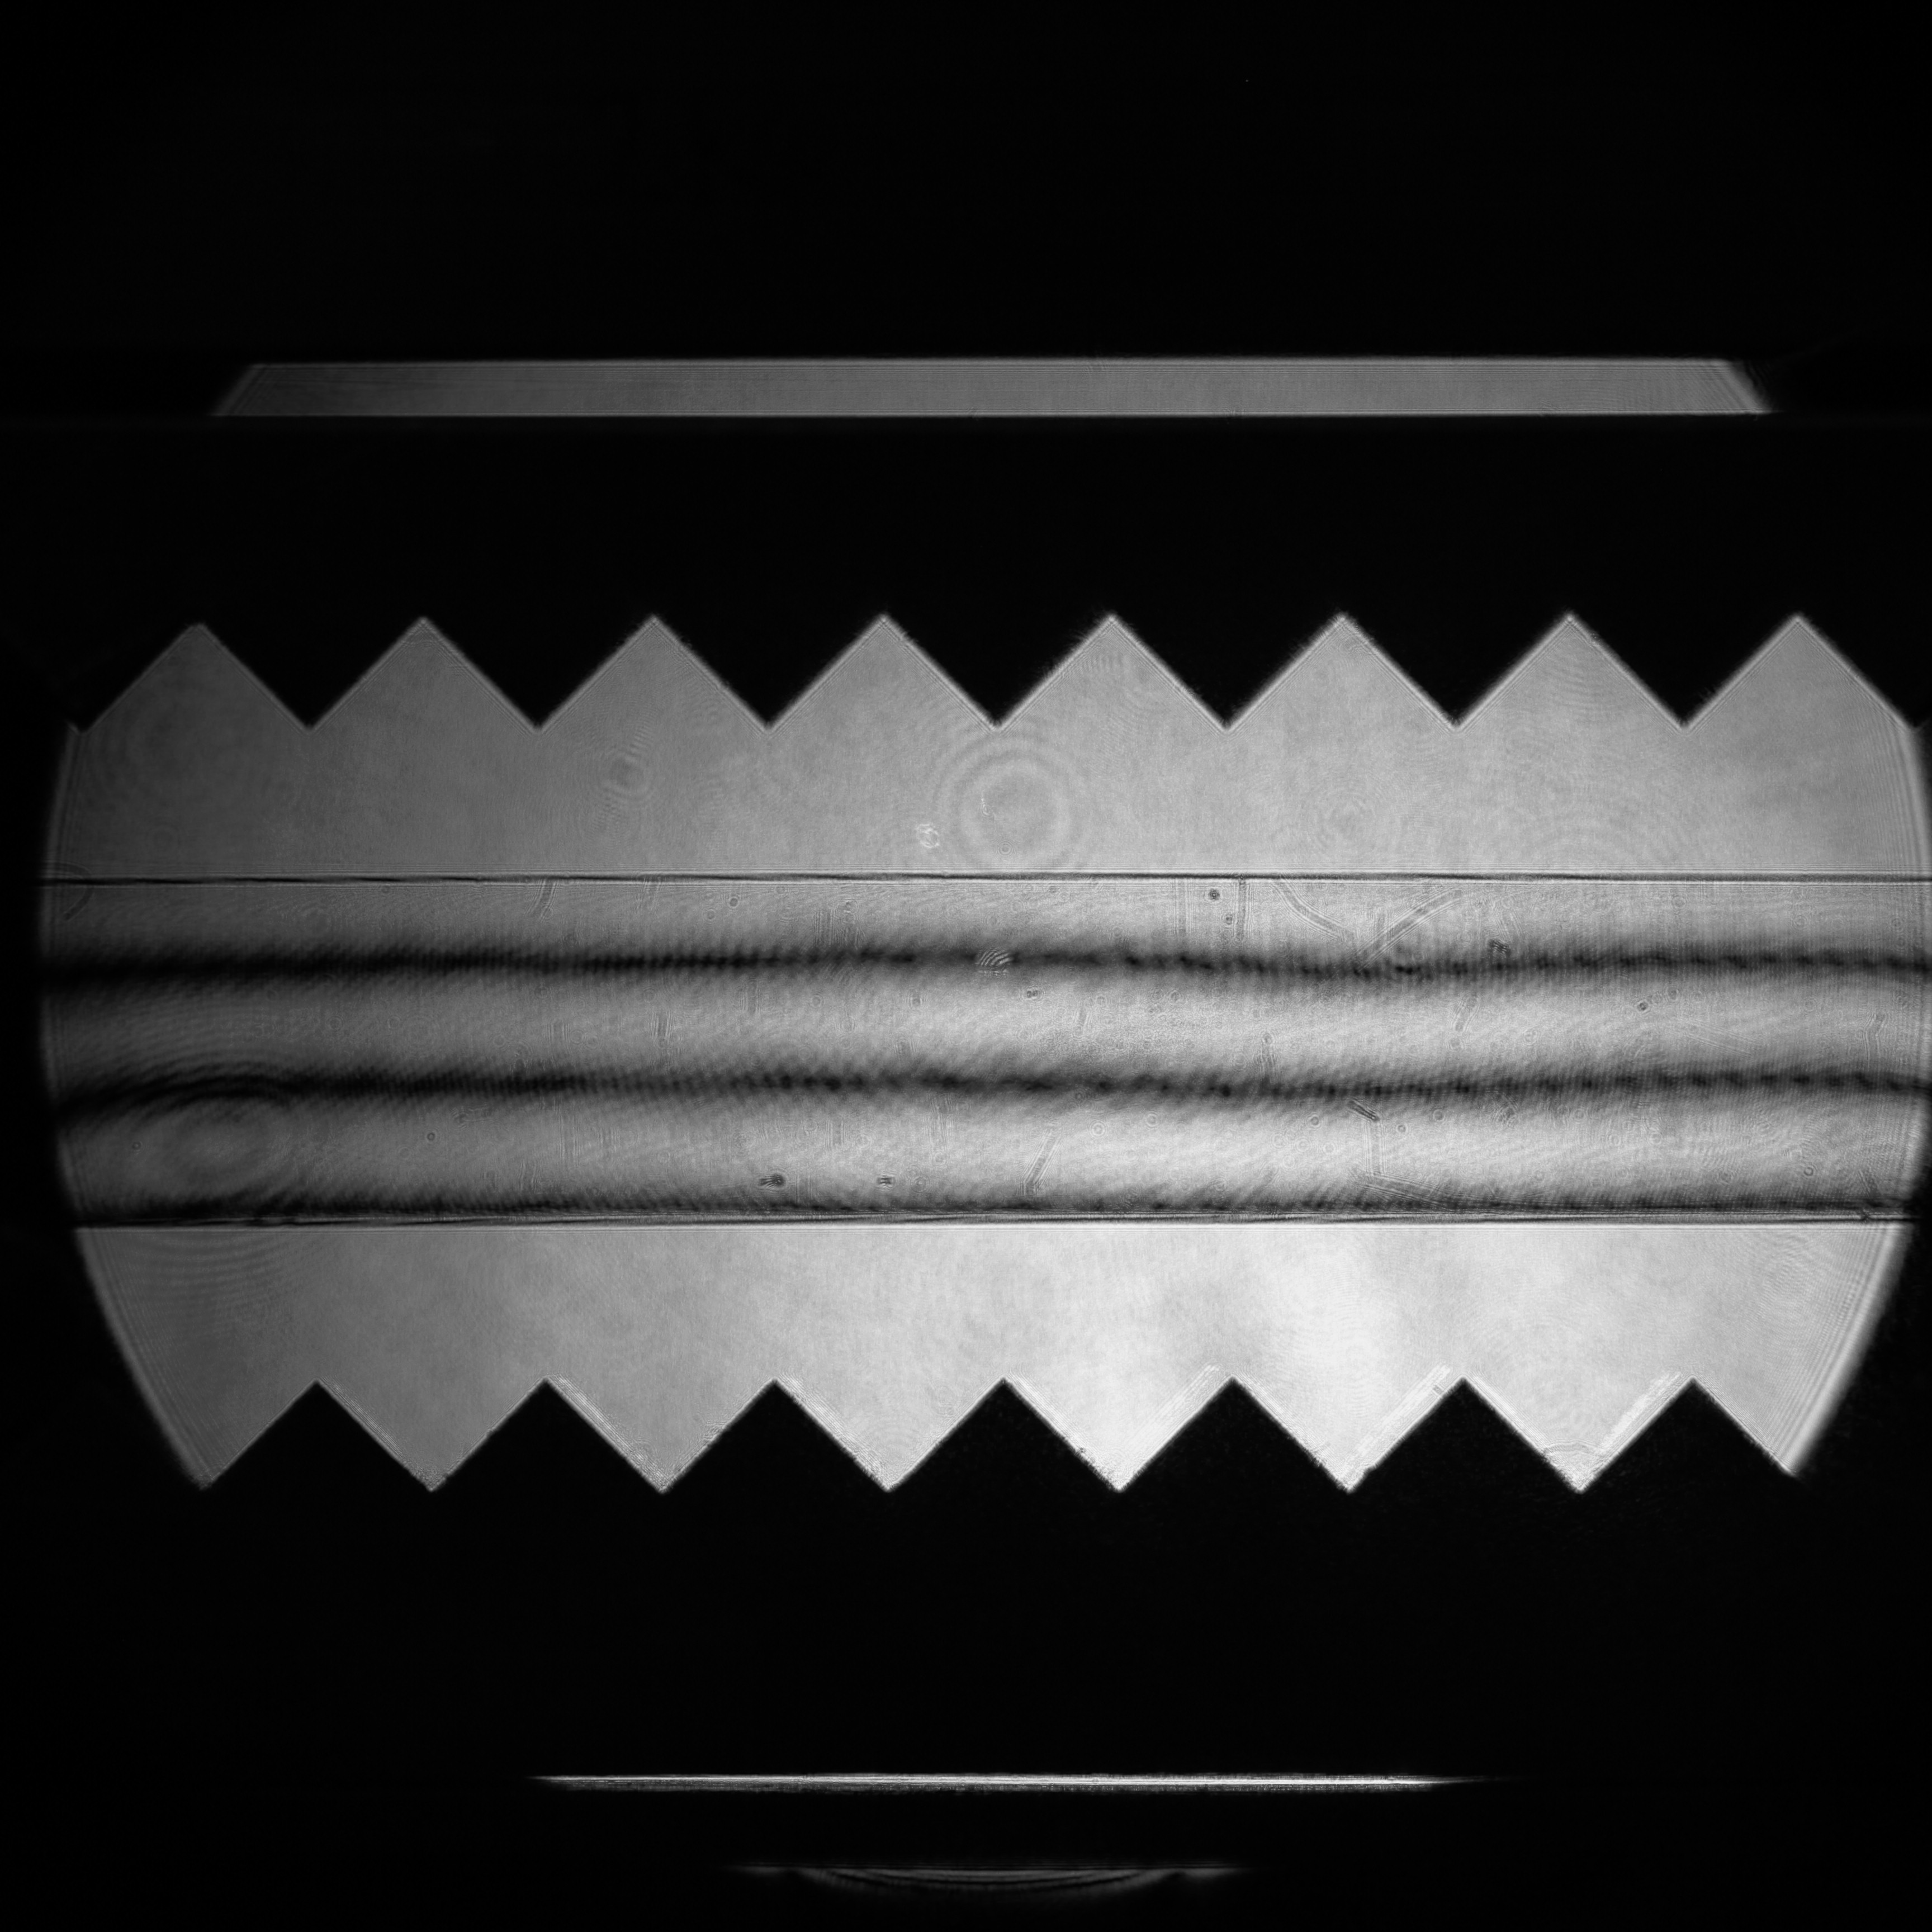
\includegraphics[width=\textwidth]{e=2,W=4.5.JPG}
        \caption{$e=2, W=4.5$ (明)}
    \end{minipage}
    \hfill
    \begin{minipage}[b]{0.48\textwidth}
        \centering
        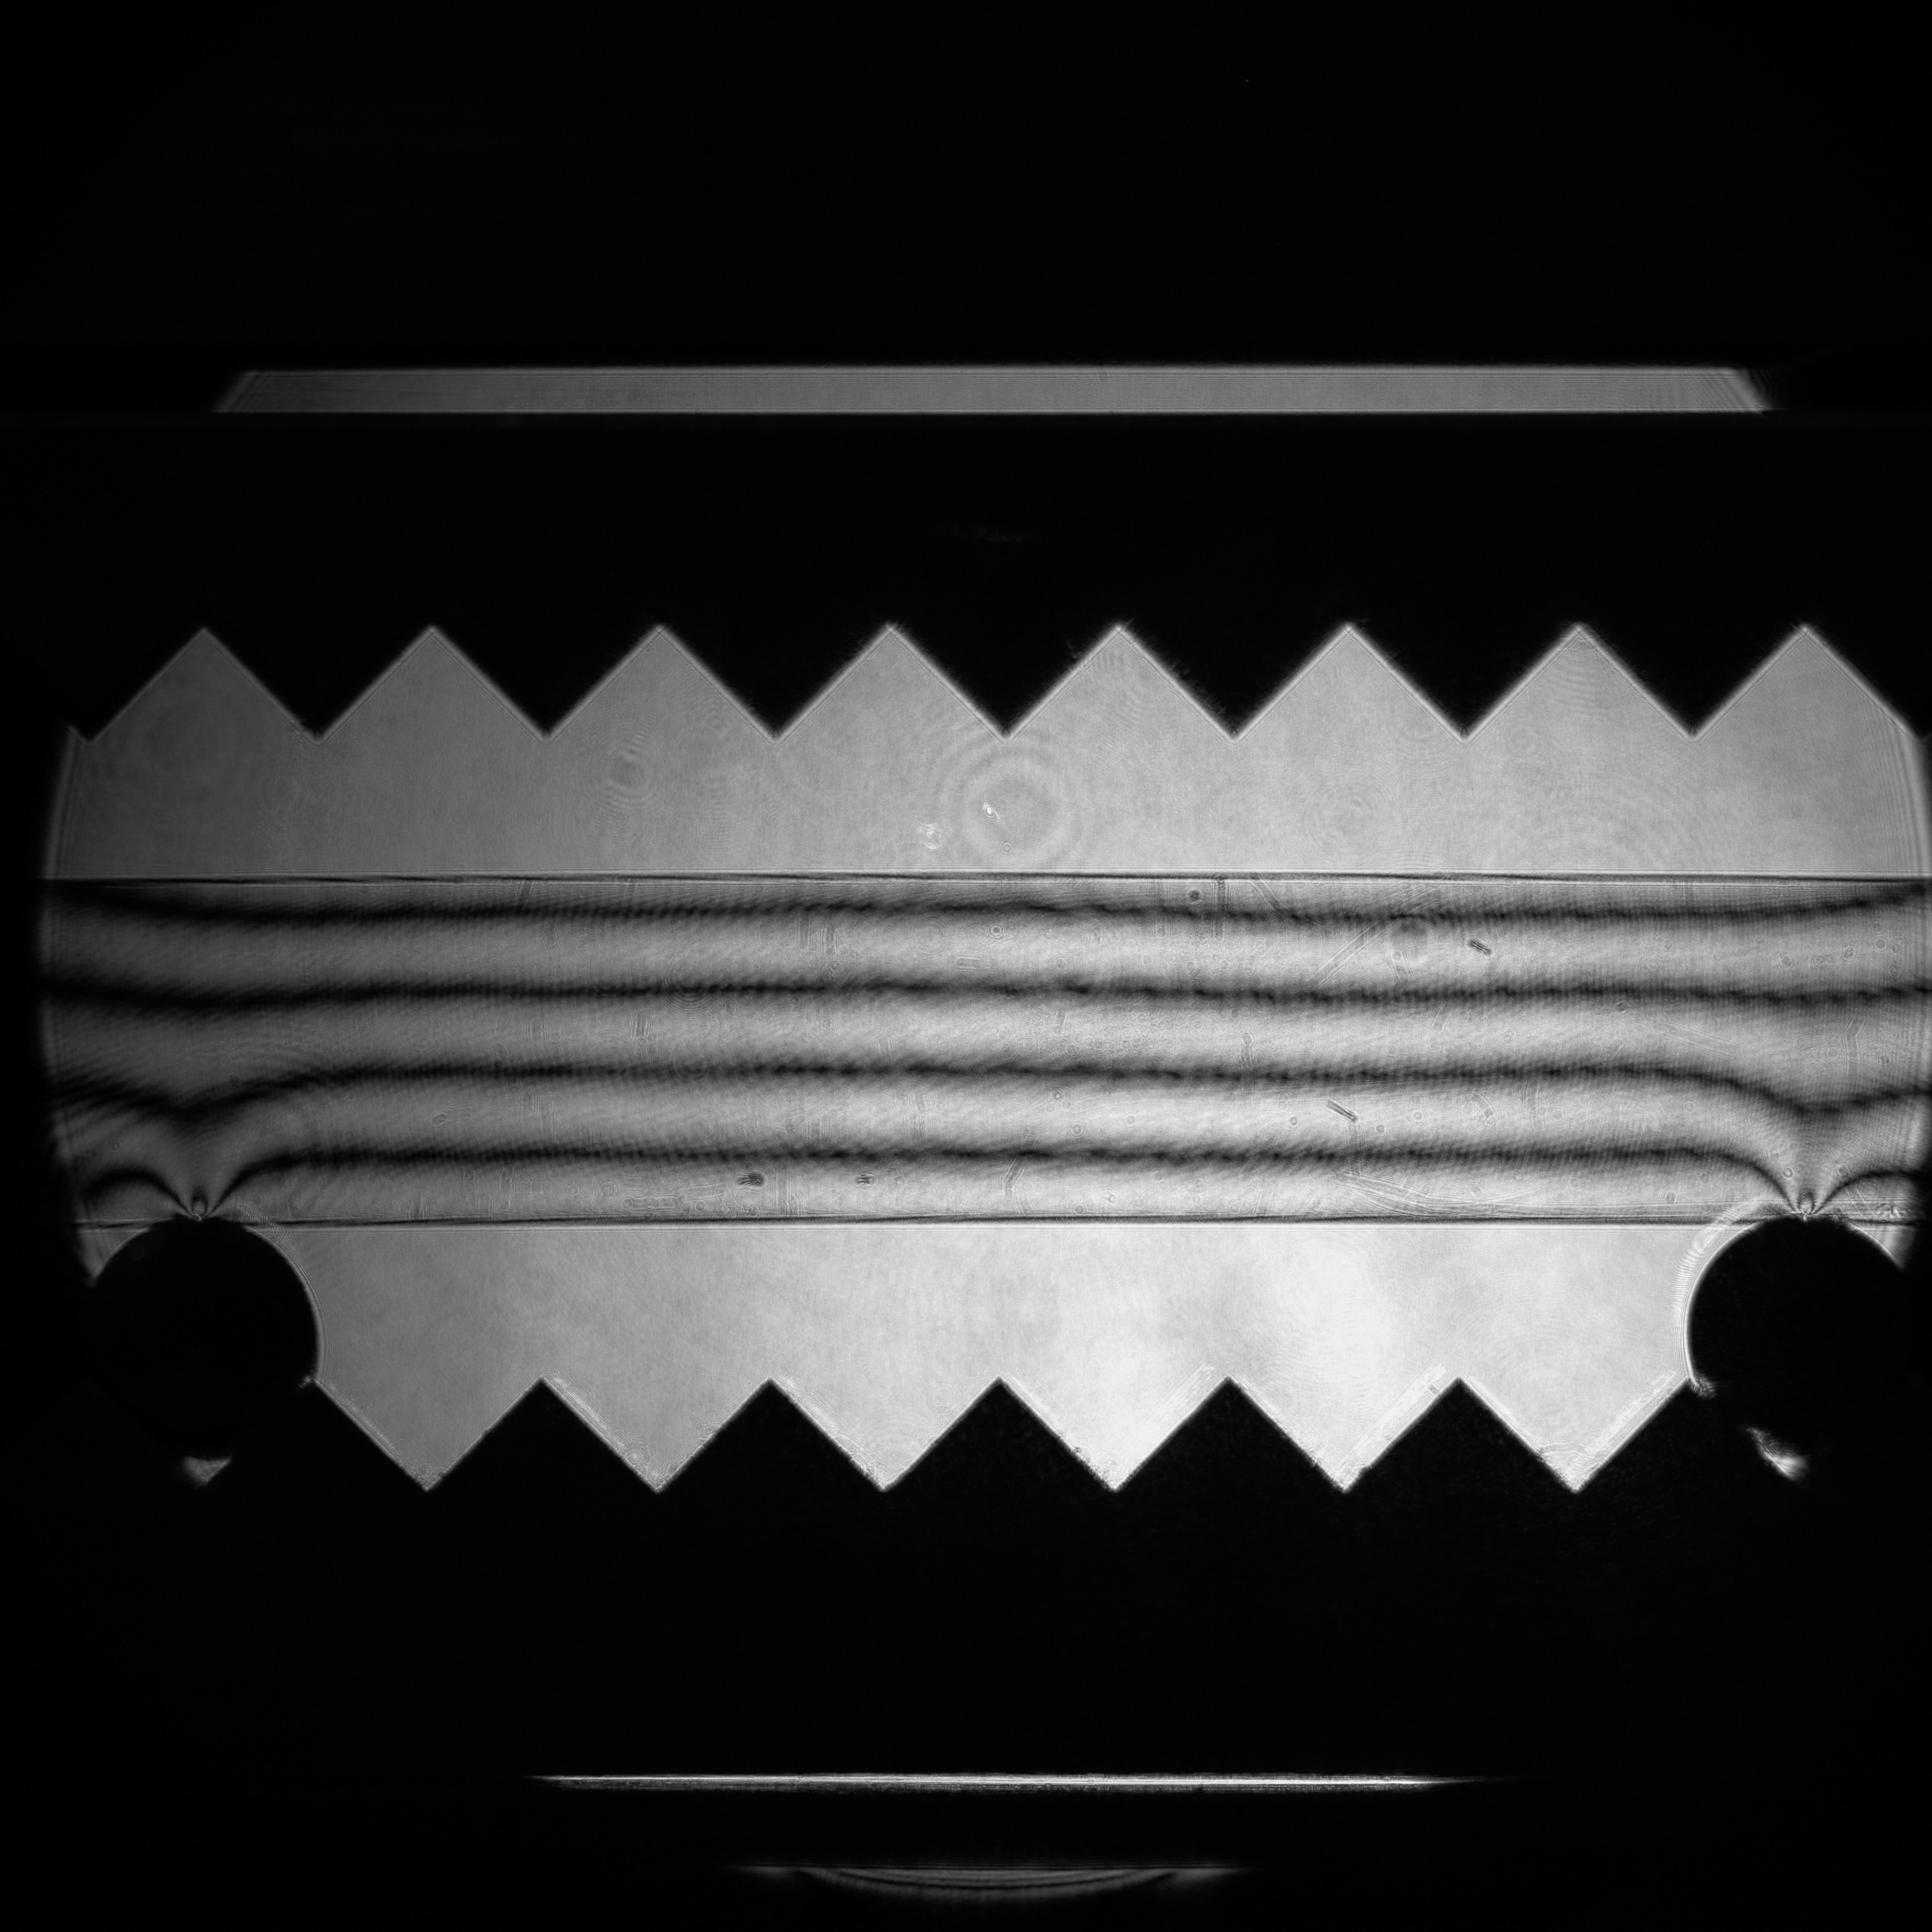
\includegraphics[width=\textwidth]{e=3,W=4.5.JPG}
        \caption{$e=3, W=4.5$ (明)}
    \end{minipage}
    \\ \vspace{5mm}
    \begin{minipage}[b]{0.48\textwidth}
        \centering
        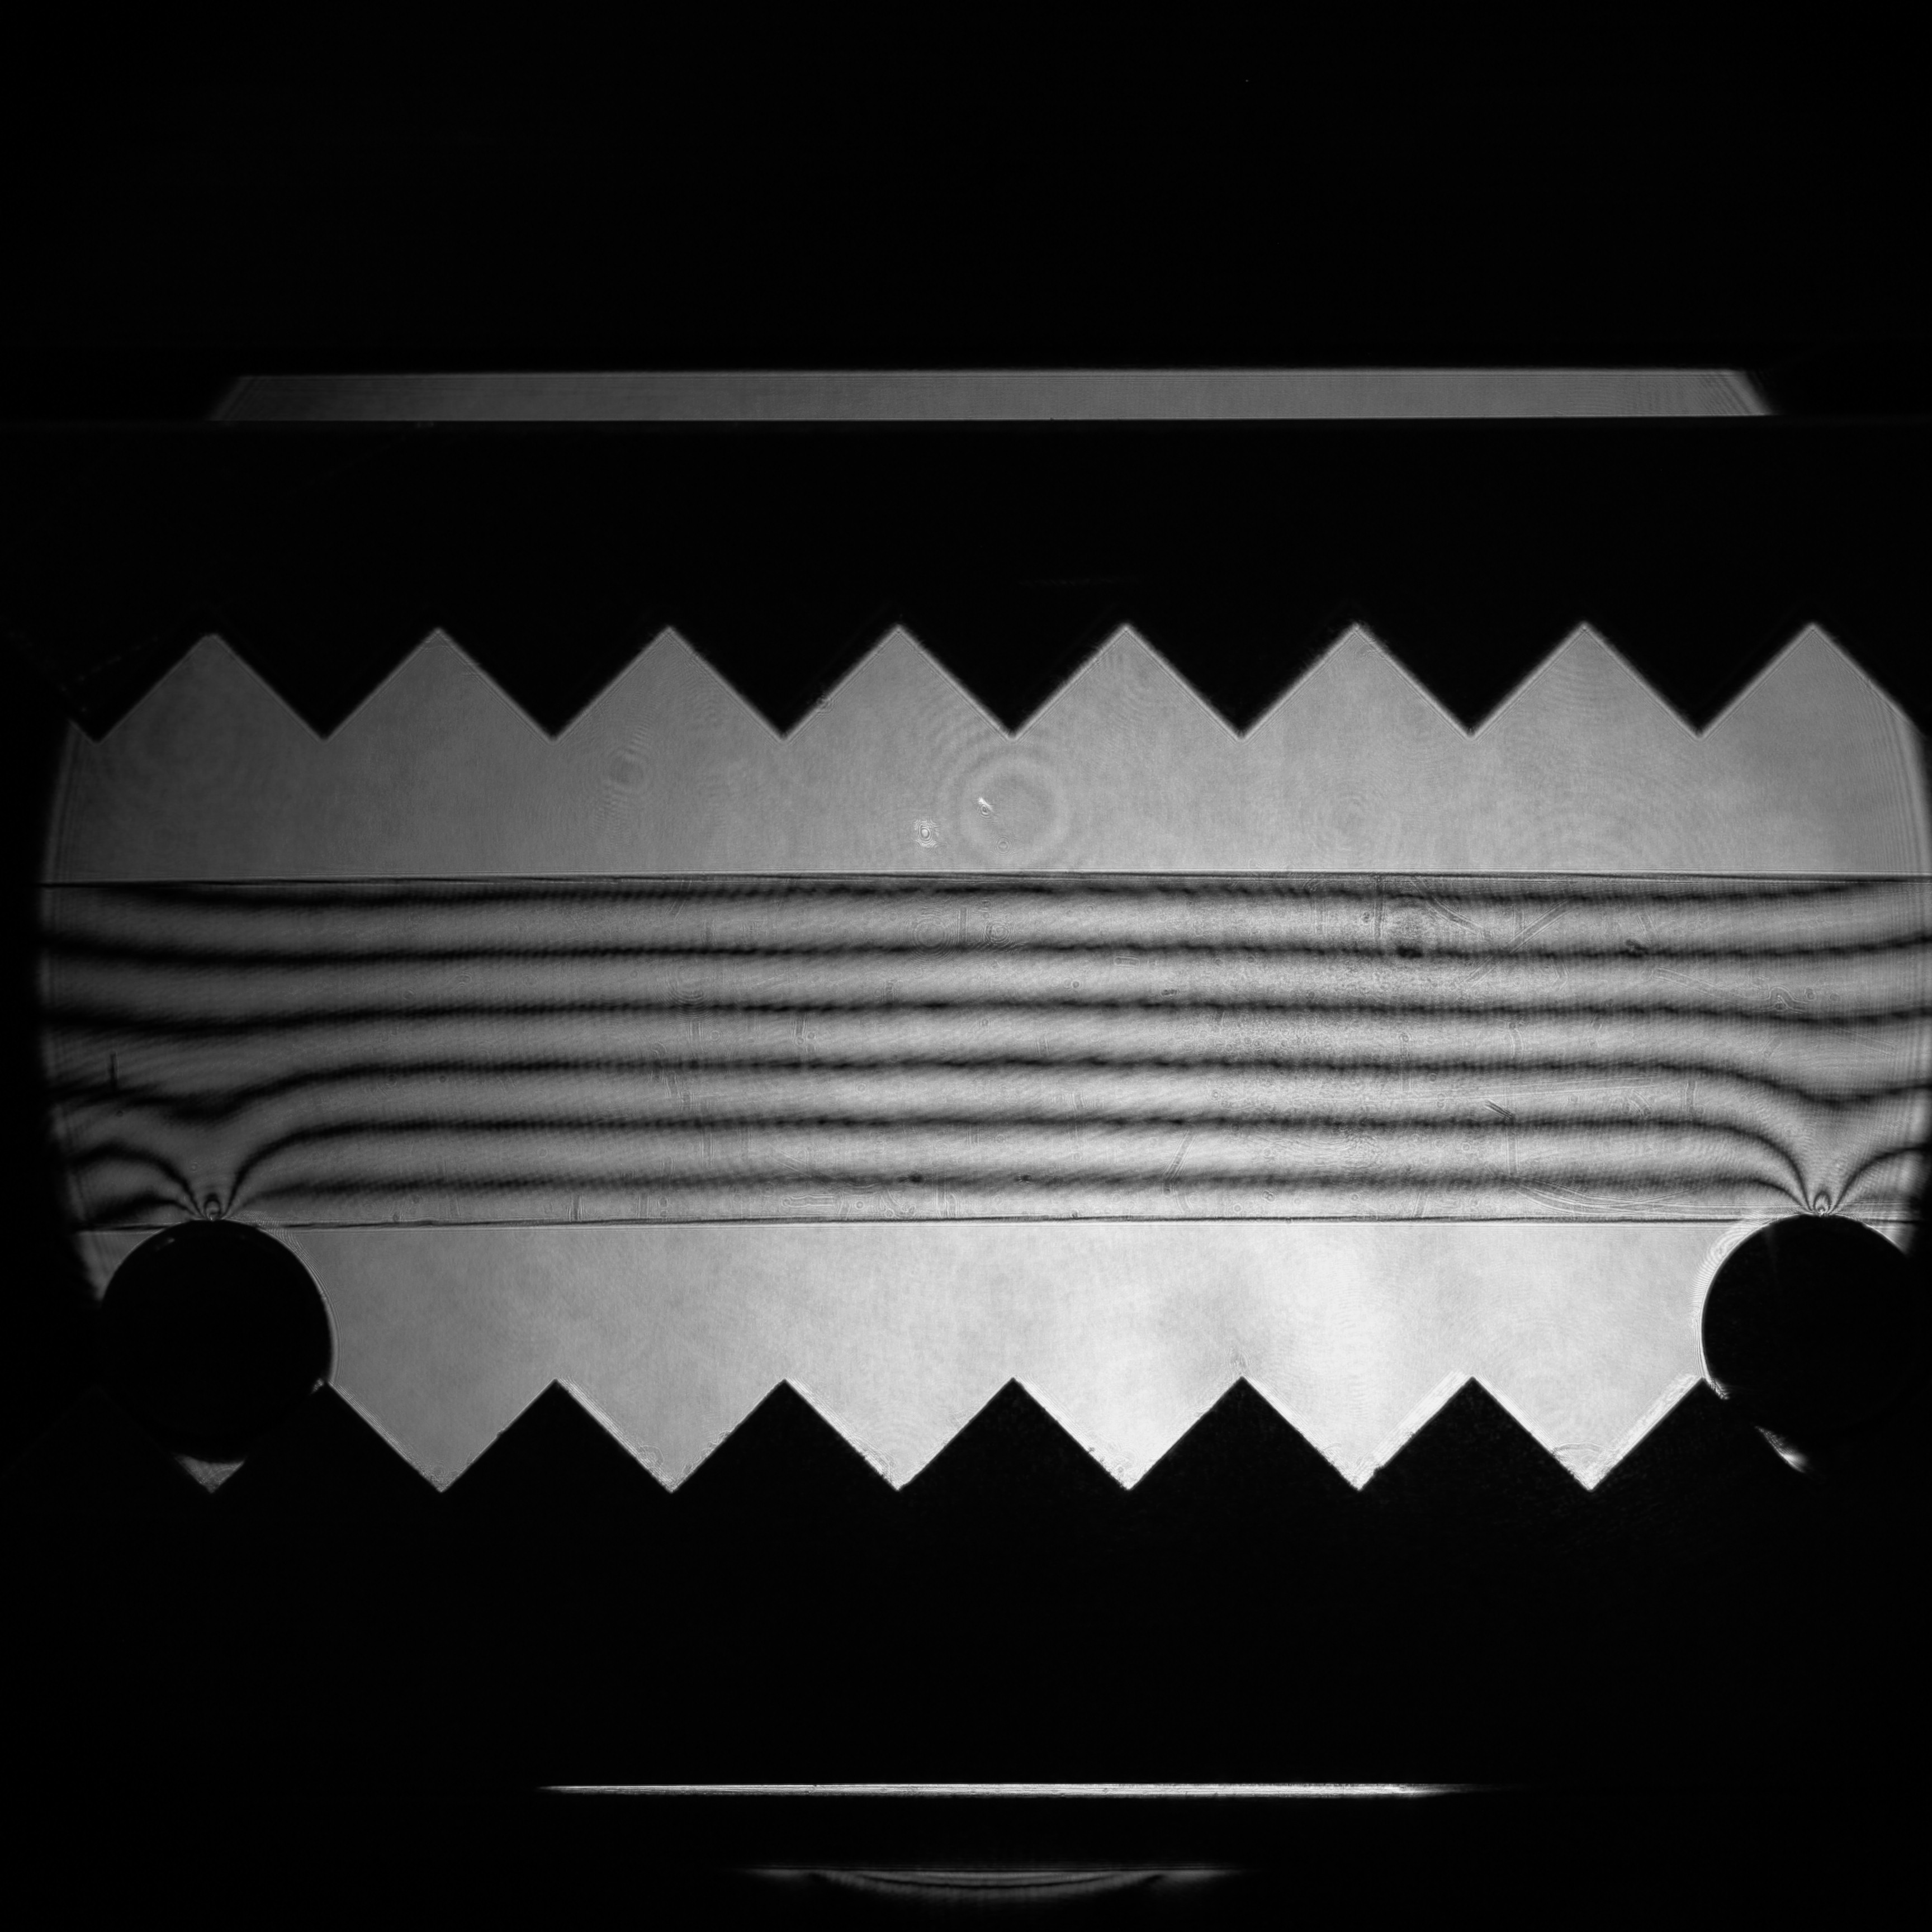
\includegraphics[width=\textwidth]{e=3,W=6.5.JPG}
        \caption{$e=3, W=6.5$ (明)}
    \end{minipage}
    \hfill
    \begin{minipage}[b]{0.48\textwidth}
        \centering
        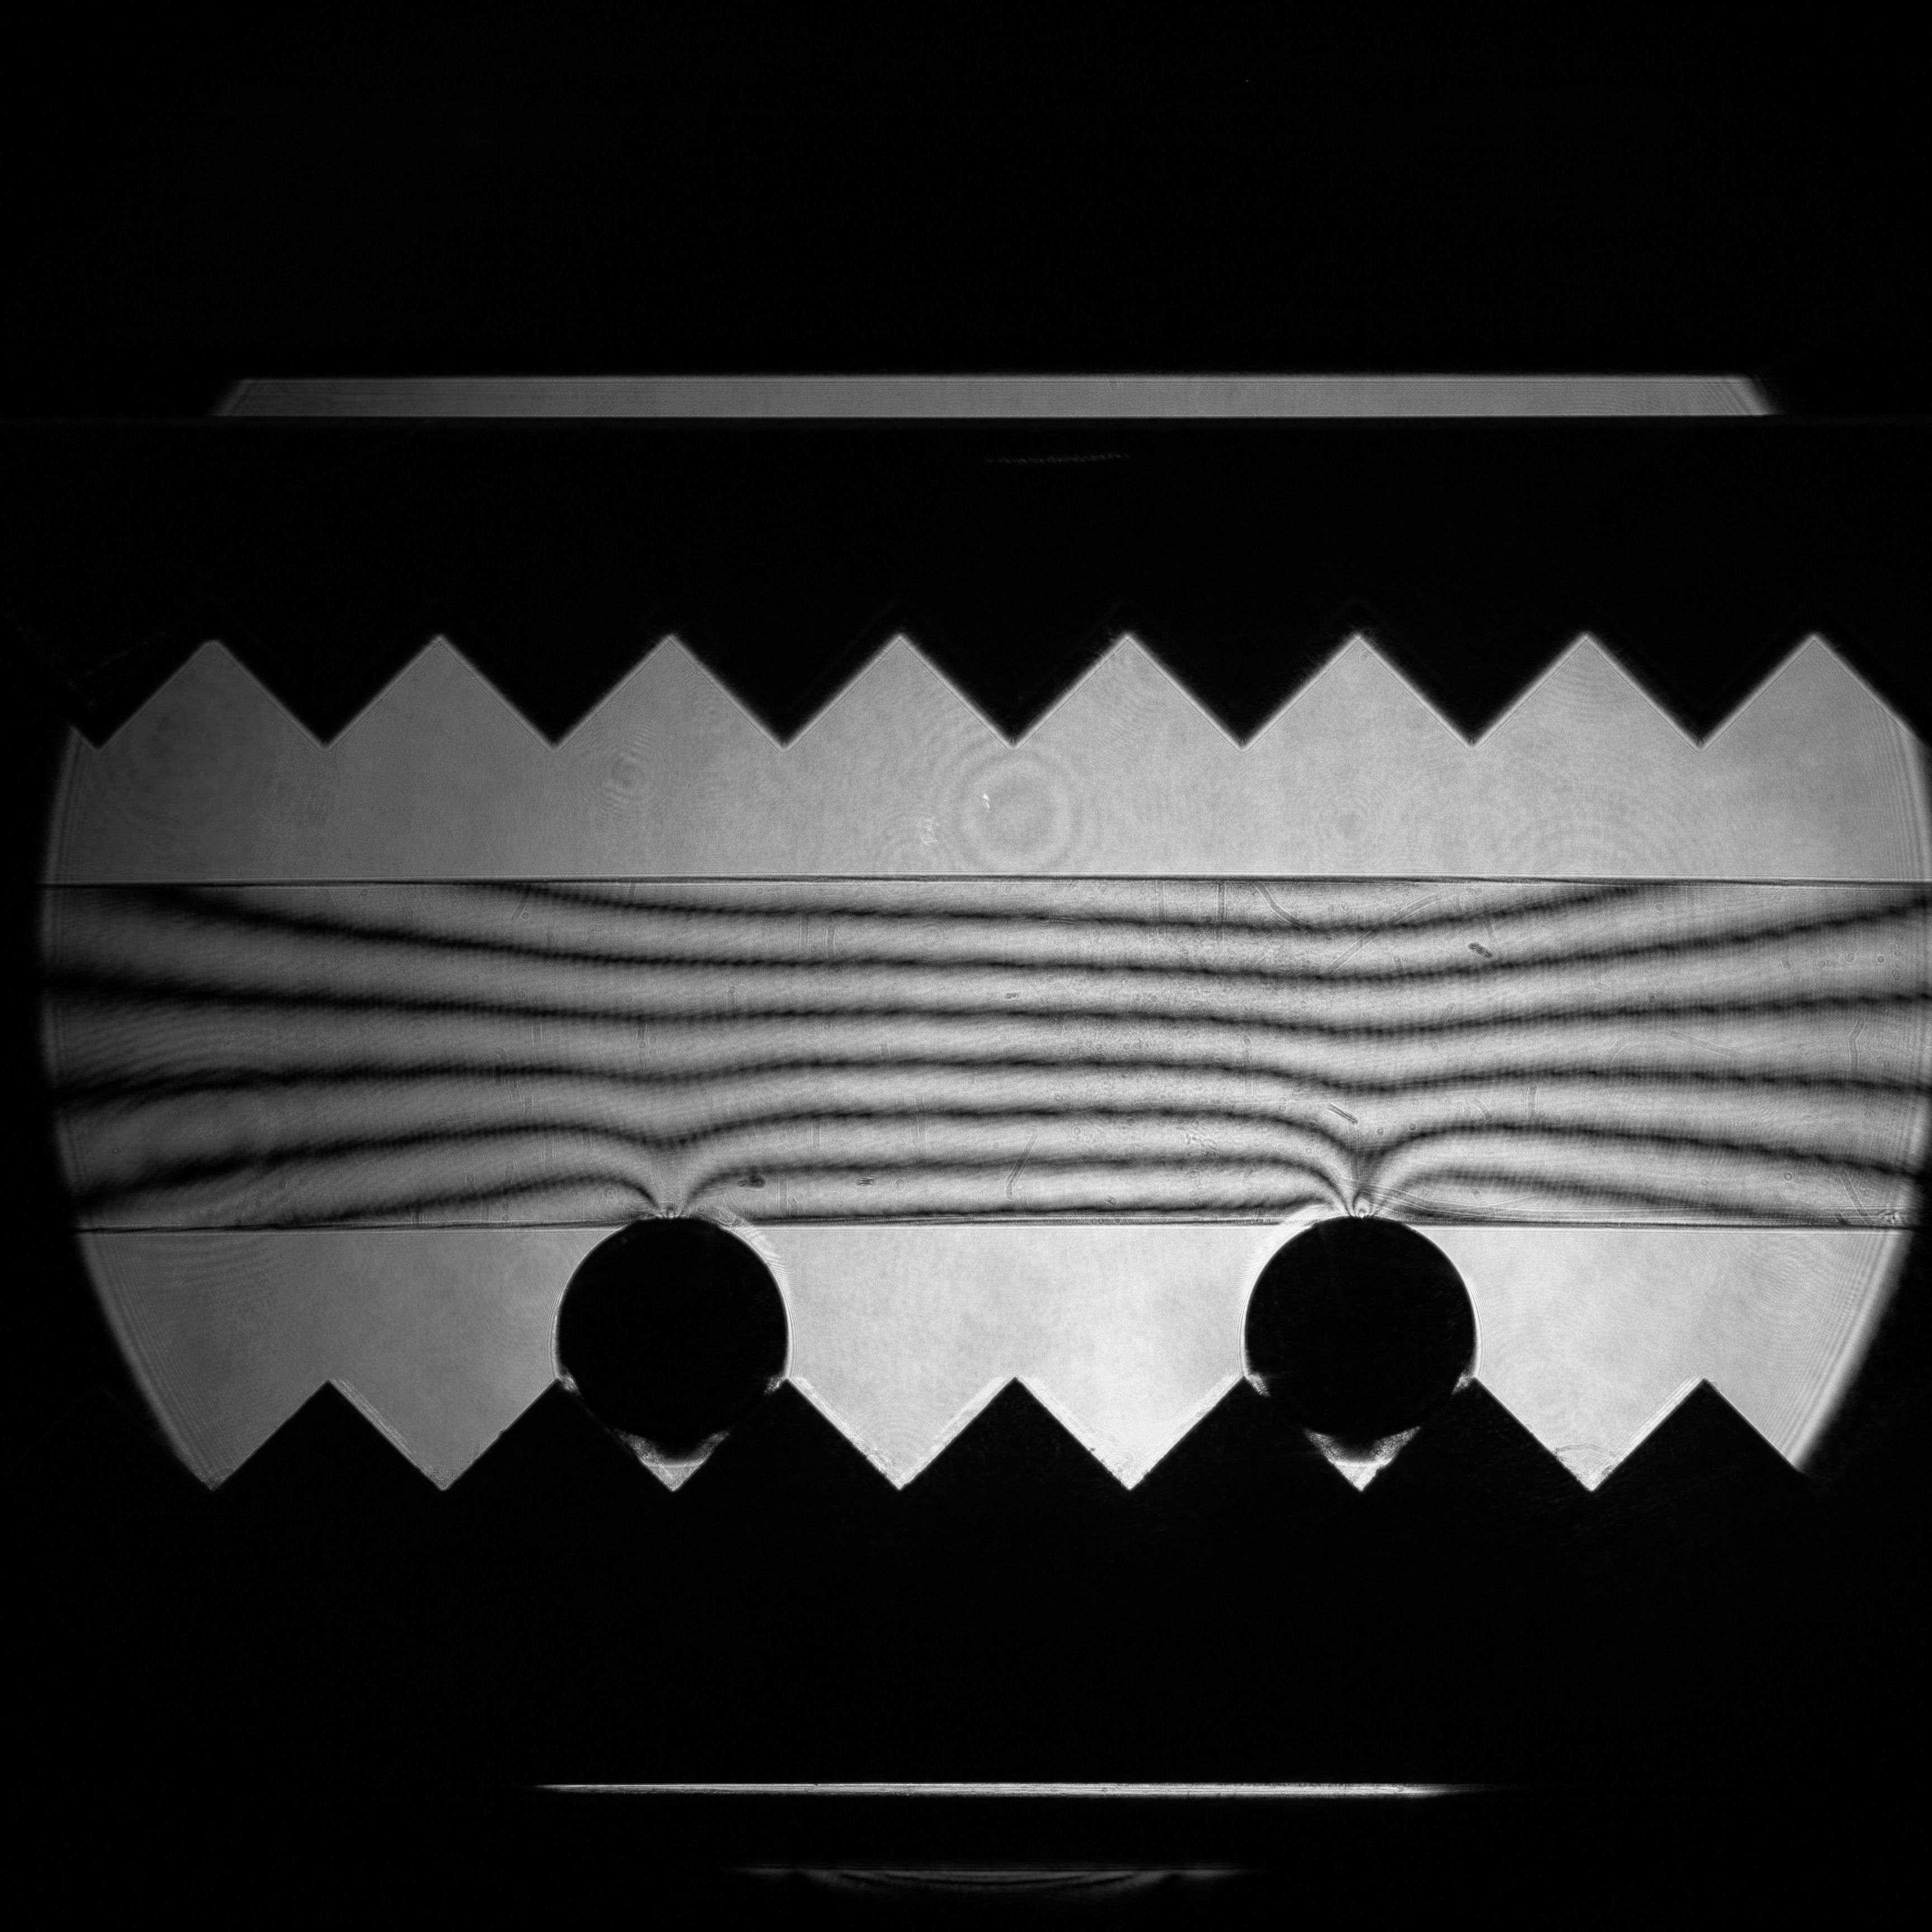
\includegraphics[width=\textwidth]{e=5,W=4.5.JPG}
        \caption{$e=5, W=4.5$ (明)}
    \end{minipage}
    \\ \vspace{5mm}
    \begin{minipage}[b]{0.48\textwidth}
        \centering
        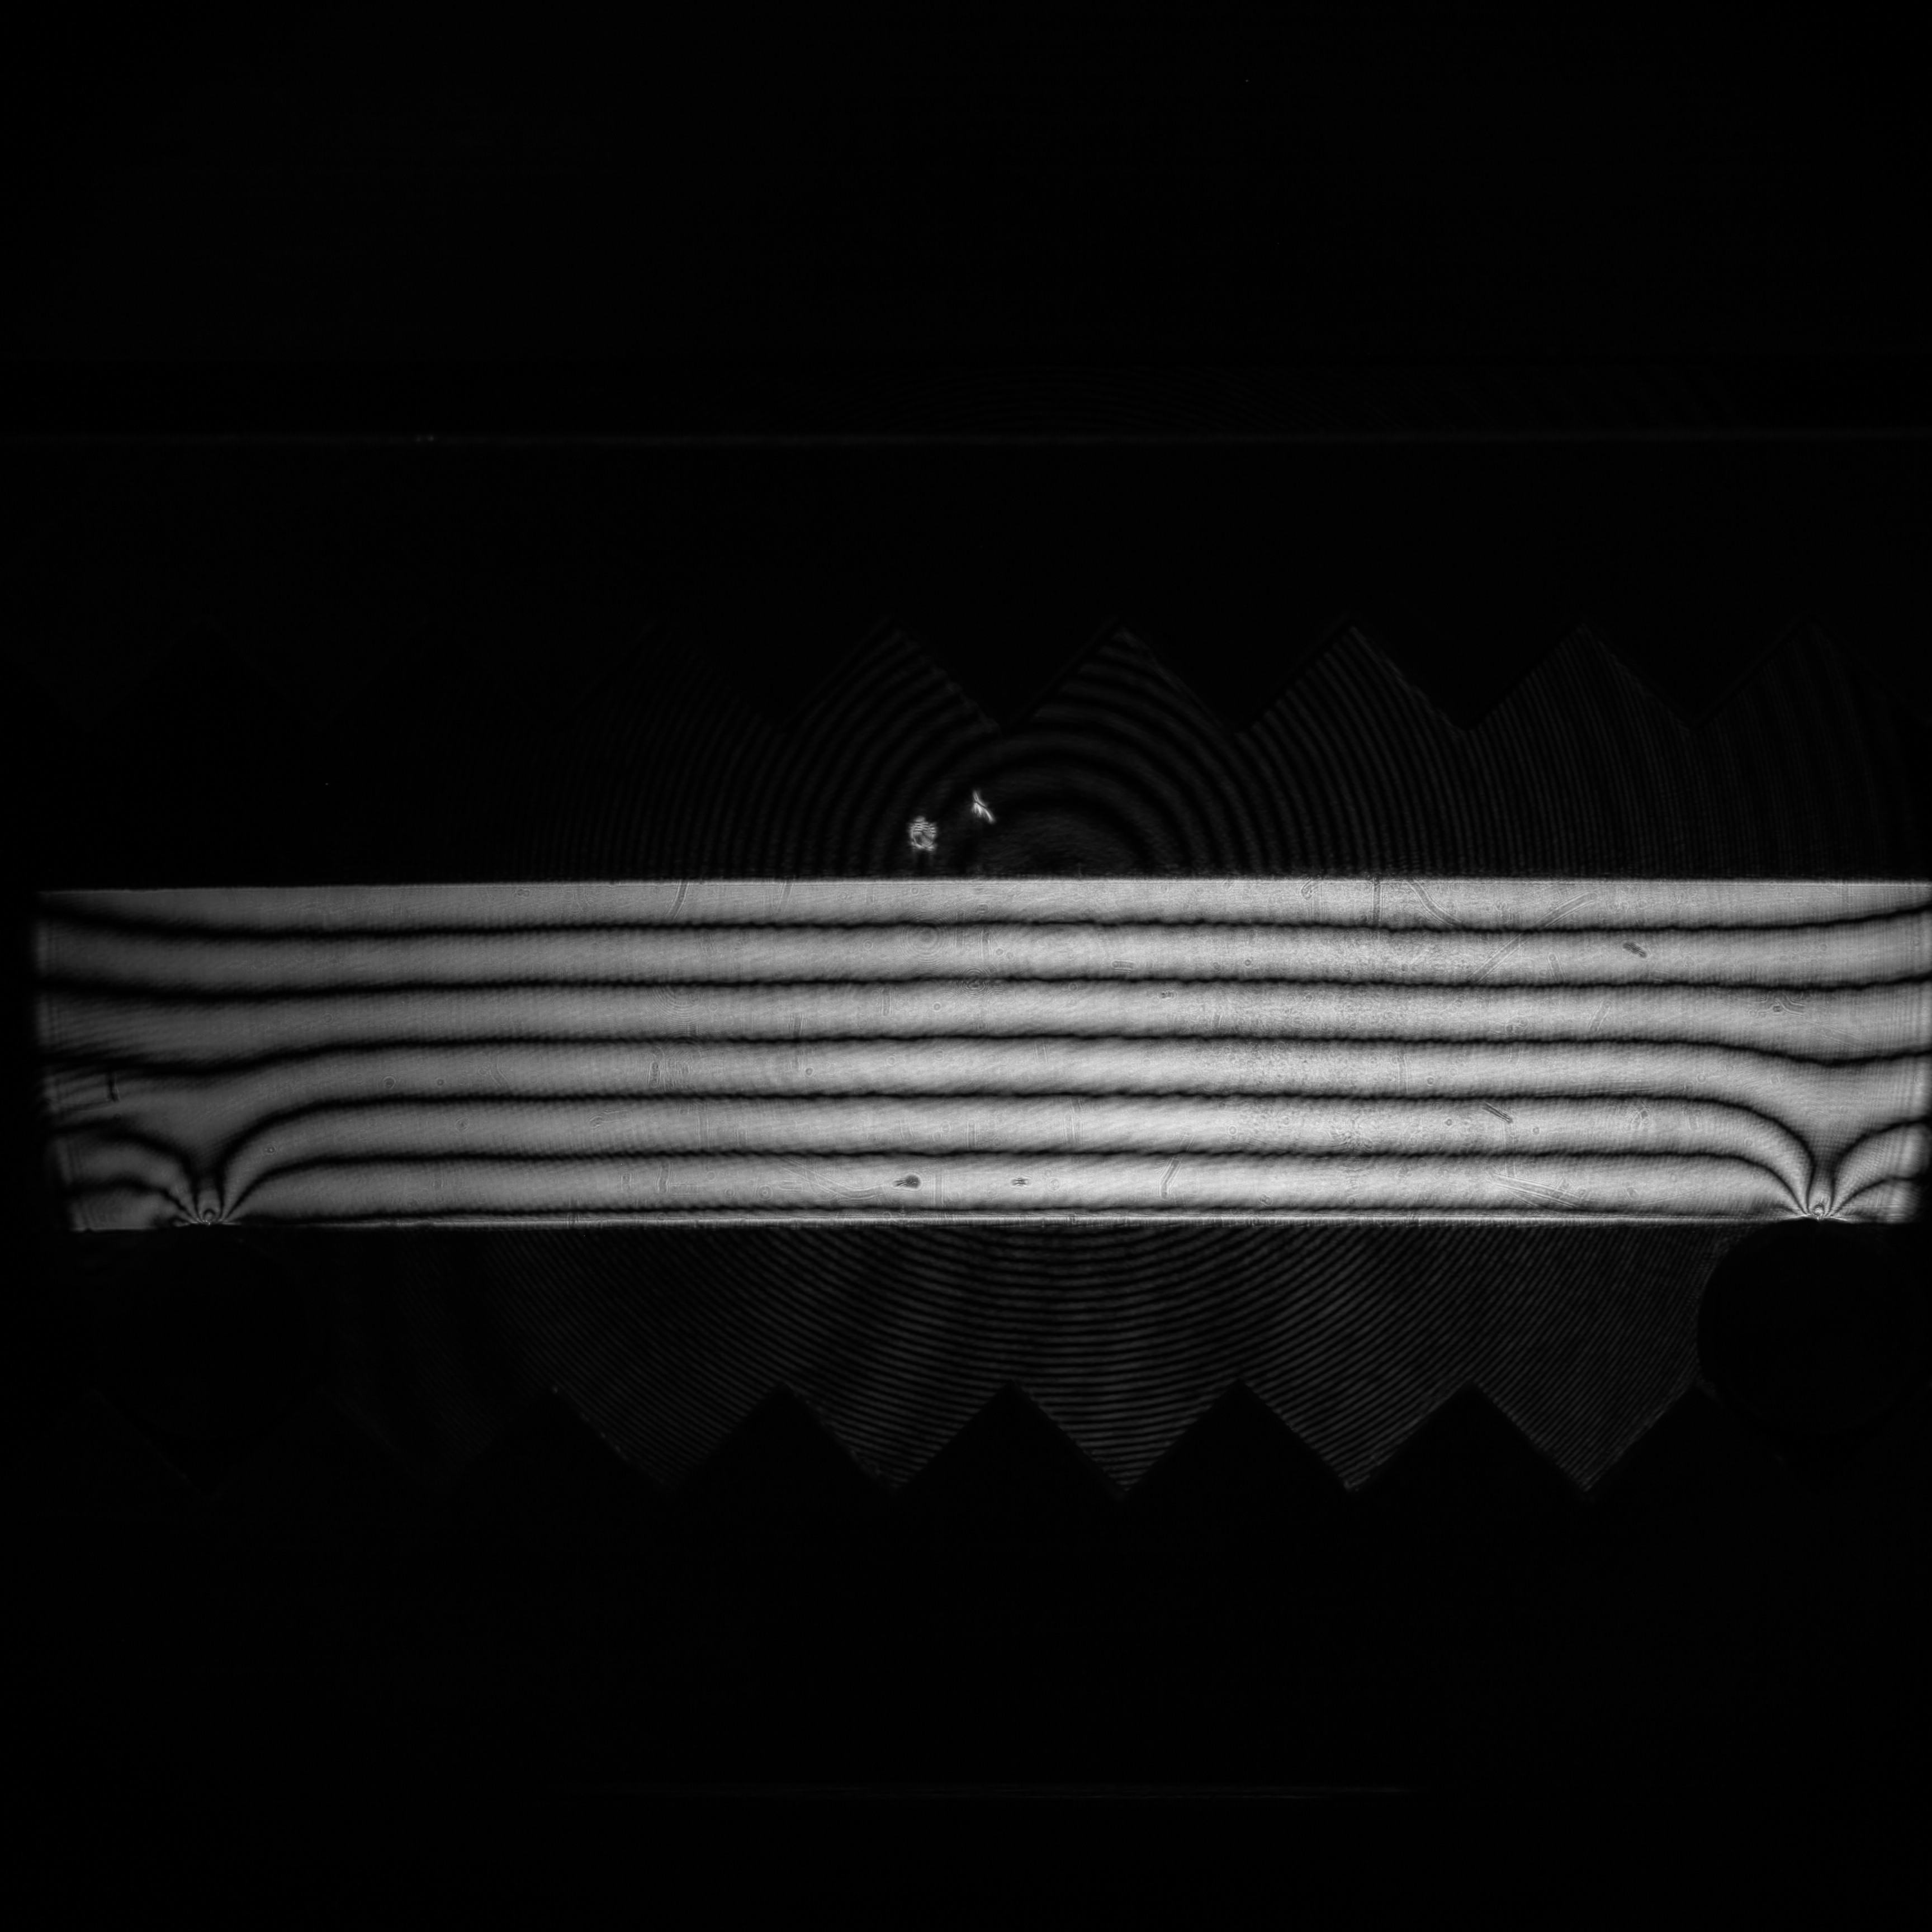
\includegraphics[width=\textwidth]{暗 e=3,W=4.5.JPG}
        \caption{$e=3, W=4.5$ (暗)}
    \end{minipage}
\end{figure}

今回の課題においては上下の$N_{\text{max}}$を測定した。\\
この測定値と配布テキストで導いた(1-23)式にある$N_{\text{max}}=3CWe/\lambda h^2$を用いて、光弾性係数$C$の値を求めた（ここで、$N_{\text{max}}$は縞次数、$W$は荷重、$\lambda$はレーザー光の波長、$h$は厚みである）。\\
$e, W$の値と、上側の縞次数によって求められる$C$の値、および下側の縞次数によってもとめられる$C$の値の関係は表1のようになった。\\
この時、中立面から上部を$N$(上)、中立面より下部を$N$(下)とし、撮影した画像においてコンピュータ上で倍率を100\%としモニター上の大きさを測定した。その後、中立面より上の最大の大きさである$N_{\text{max}}$の値を、モニター上の1目盛分の大きさで割ることによって縞次数を求めた。

\begin{table}[H]
\centering
\caption{各条件における縞次数と光弾性係数$C$の算出結果}
\resizebox{\textwidth}{!}{
\begin{tabular}{cccccccccccc}
\hline
明暗 & $W$(kg) & $e$(cm) & $N_{\text{max}}$(上) & $N_{\text{max}}$(下) & 1目盛の長さ & $N_{\text{max}}$(上)  & $N_{\text{max}}$(下)  & $C$(上)     & $C$(下)     & $C_{\text{Br}}$(上) & $C_{\text{Br}}$(下) \\ \hline
明  & 4.5   & 2     & 4.3     & 6.8     & 6.2       & 1.19 & 1.60 & 6.42E-11 & 8.59E-11 & 64.22    & 85.92    \\
明  & 4.5   & 3     & 5.5     & 7.4     & 4.2       & 1.81 & 2.26 & 6.49E-11 & 8.11E-11 & 64.91    & 81.14    \\
明  & 4.5   & 5     & 6.7     & 10.3    & 2.5       & 3.18     & 4.62     & 6.84E-11 & 9.94E-11 & 68.45    & 99.44    \\
明  & 6.5   & 3     & 6.5     & 10.5    & 2.8       & 2.82 & 4.25     & 7.01E-11 & 1.06E-10 & 70.07    & 105.55   \\
暗  & 6.5   & 3     & 7.6     & 9       & 2.8       & 2.71 & 3.21 & 6.74E-11 & 7.98E-11 & 67.41    & 79.83    \\ \hline
\end{tabular}
}
\end{table}

また、上部の縞次数に対する$C_{\text{Br}}$の平均は67.0、下部の縞次数に対する$C_{\text{Br}}$の平均は90.38となった。\\
これらにはかなりの差があるといえる。この理由として以下のことが考えられる。
\begin{enumerate}[label=\arabic*.]
    \item 画像上では縞が幅をもってしまうため、正確な縞の位置を測定するのが難しいこと。
    \item 中立面が梁の完全な幾何学的中心とはなっていないこと。% TO DO: この点について後段で追記
    \item 支点や荷重を加えるピン自体に有限の大きさがあること。
    \item 支点の三次元的なずれから、三次元的な力が加わっている可能性があること。
\end{enumerate}

$e=2, W=4.5$の光弾性画像と、$e=3, W=4.5$の光弾性画像を比較すると、$e=3, W=4.5$の条件においてより$N_{\text{max}}$の値が大きくなっていることがわかる。また、$e=3, W=4.5$の光弾性画像と$e=3, W=6.5$の光弾性画像を比較すると、$e=3, W=6.5$の条件においてより$N_{\text{max}}$の値が大きくなっていることがわかる。\\
これはテキスト(1-23)式の$N_{\text{max}}=3CWe/\lambda h^2$より、$W, e$が大きくなると$N_{\text{max}}$が大きくなることから明らかである。

課題2における荷重条件を検討するにあたっては、以下の点を考慮した。
\begin{itemize}
    \item 荷重が加わる点については縞模様が歪むため、中心付近（つまり$e$が大きい状態）で荷重が加わるのは好ましくない。
    \item 一方で$e, W$の値が小さい状態では、$N_{\text{max}}$の測定に大きな誤差を含んでしまうため好ましくない。
    \item $e, W$が大きすぎる場合、切り欠き部分に多くの縞の重なりが生じ、適切に値を読み取ることができない。
\end{itemize}
これらのことを考慮した結果、条件として$e=3, W=6.5$を採用した。

$e=3, W=4.5$について暗視野と明視野を比較すると、それぞれの利点と問題点は以下のようになった。\\
暗視野の利点は、$N=0, 1, 2\dots$に縞が現れるため中心軸の位置が分かりやすい点である。一方で問題点としては、試験片の境界が暗いため、端の値については正確な観測が難しい点が挙げられる。\\
明視野の利点は、背景が明るいため試験片の端の縞が見やすい点である。一方で問題点としては、本実験では中心軸が試験片の完全な中心ではないため、$N=1/2$の位置を探すのがより難しくなっている点が挙げられる。

\subsubsection*{課題2}
切り欠きの半径$\rho=1, 2, 4, 8$をもつ切り欠き付きの試験片に対して、課題1において検討した荷重条件（$e=3, W=6.5$）を課し、光弾性画像を撮影した。この際、明視野で実験を行った。\\
この時の$\rho$と上限の$N_{\text{max}}$、下限の$N_{\text{max}}$の関係は表2のようになった。

\begin{table}[H]
\centering
\caption{各切り欠き半径に対する$N_{\text{max}}$の測定値}
\begin{tabular}{ccc}
\hline
切欠き半径 $\rho$ (m) & $N_{\text{max}}$(下限) & $N_{\text{max}}$(上限) \\ \hline
$8.00 \times 10^{-3}$ & 4        & 4.3      \\
$4.00 \times 10^{-3}$ & 4.4      & 4.4      \\
$2.00 \times 10^{-3}$ & 5.4      & 5.5      \\
$1.00 \times 10^{-3}$ & 5.6      & 7        \\ \hline
\end{tabular}
\end{table}

また、$\rho=1, 2, 4, 8$の切り欠き付き試験片における光弾性画像は以下のようになった。
\begin{figure}[H]
    \centering
    \begin{minipage}[b]{0.48\textwidth}
        \centering
        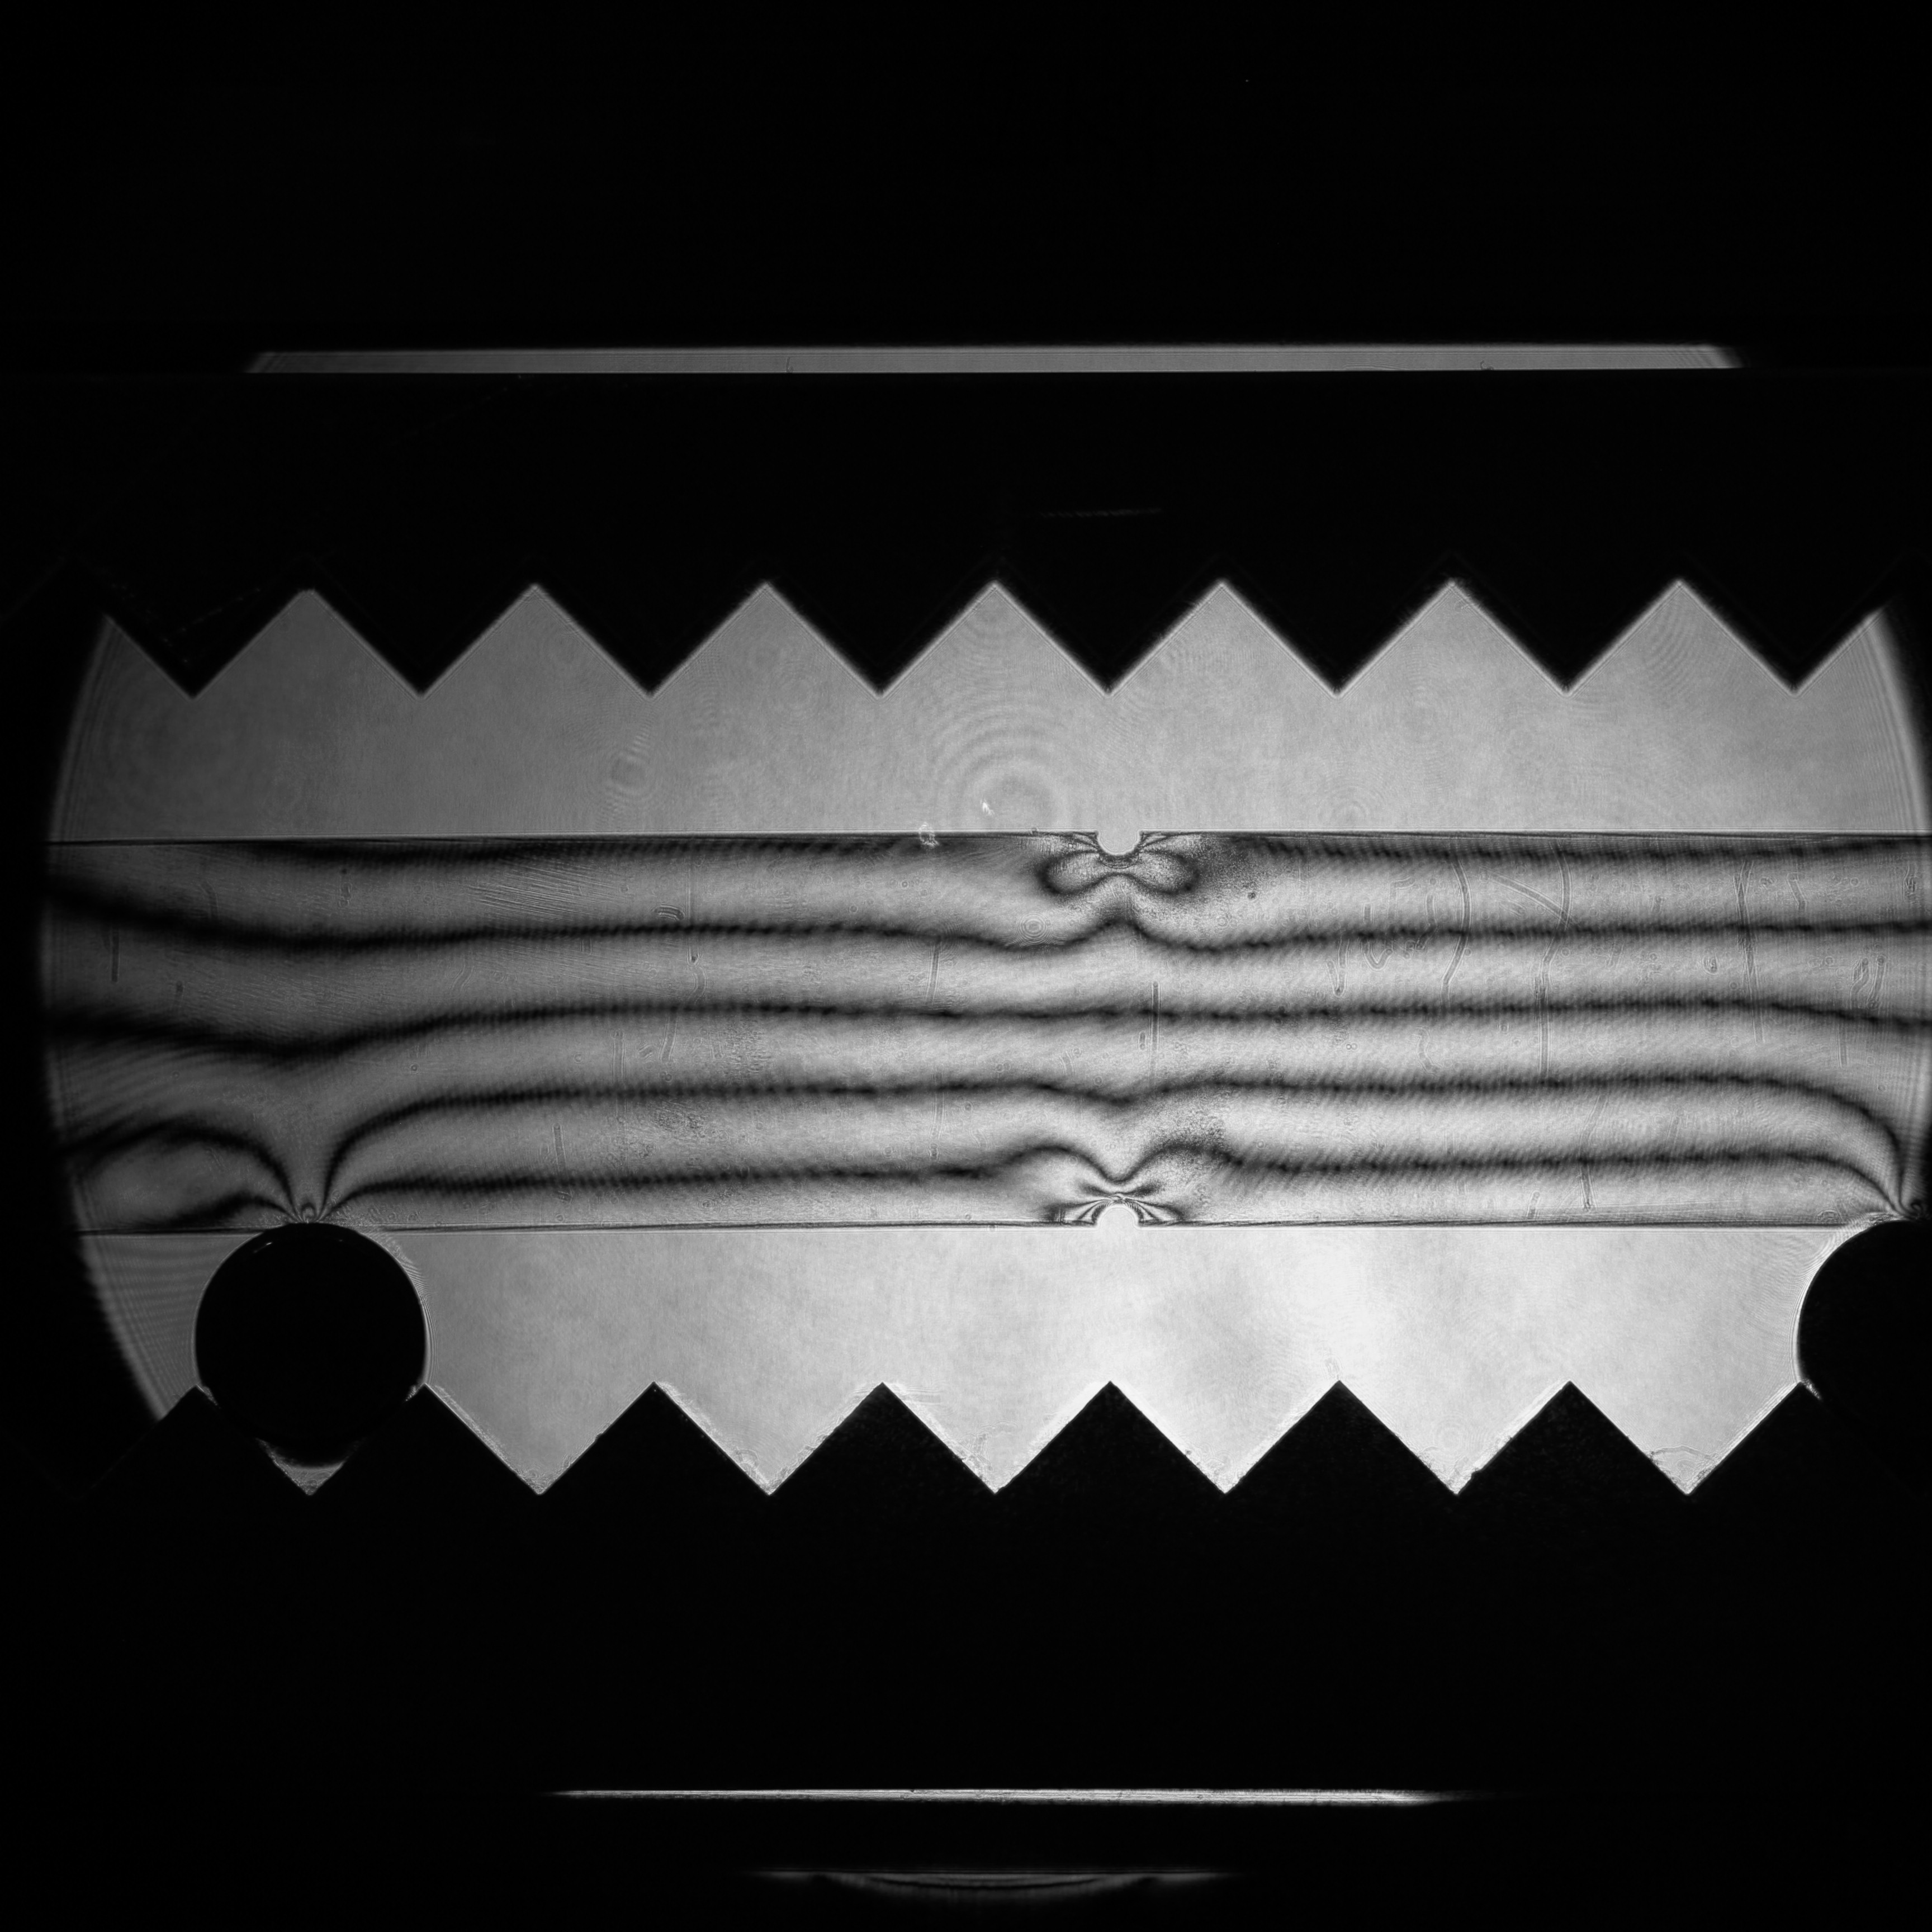
\includegraphics[width=\textwidth]{ρ=1.JPG}
        \caption{$\rho=1$}
    \end{minipage}
    \hfill
    \begin{minipage}[b]{0.48\textwidth}
        \centering
        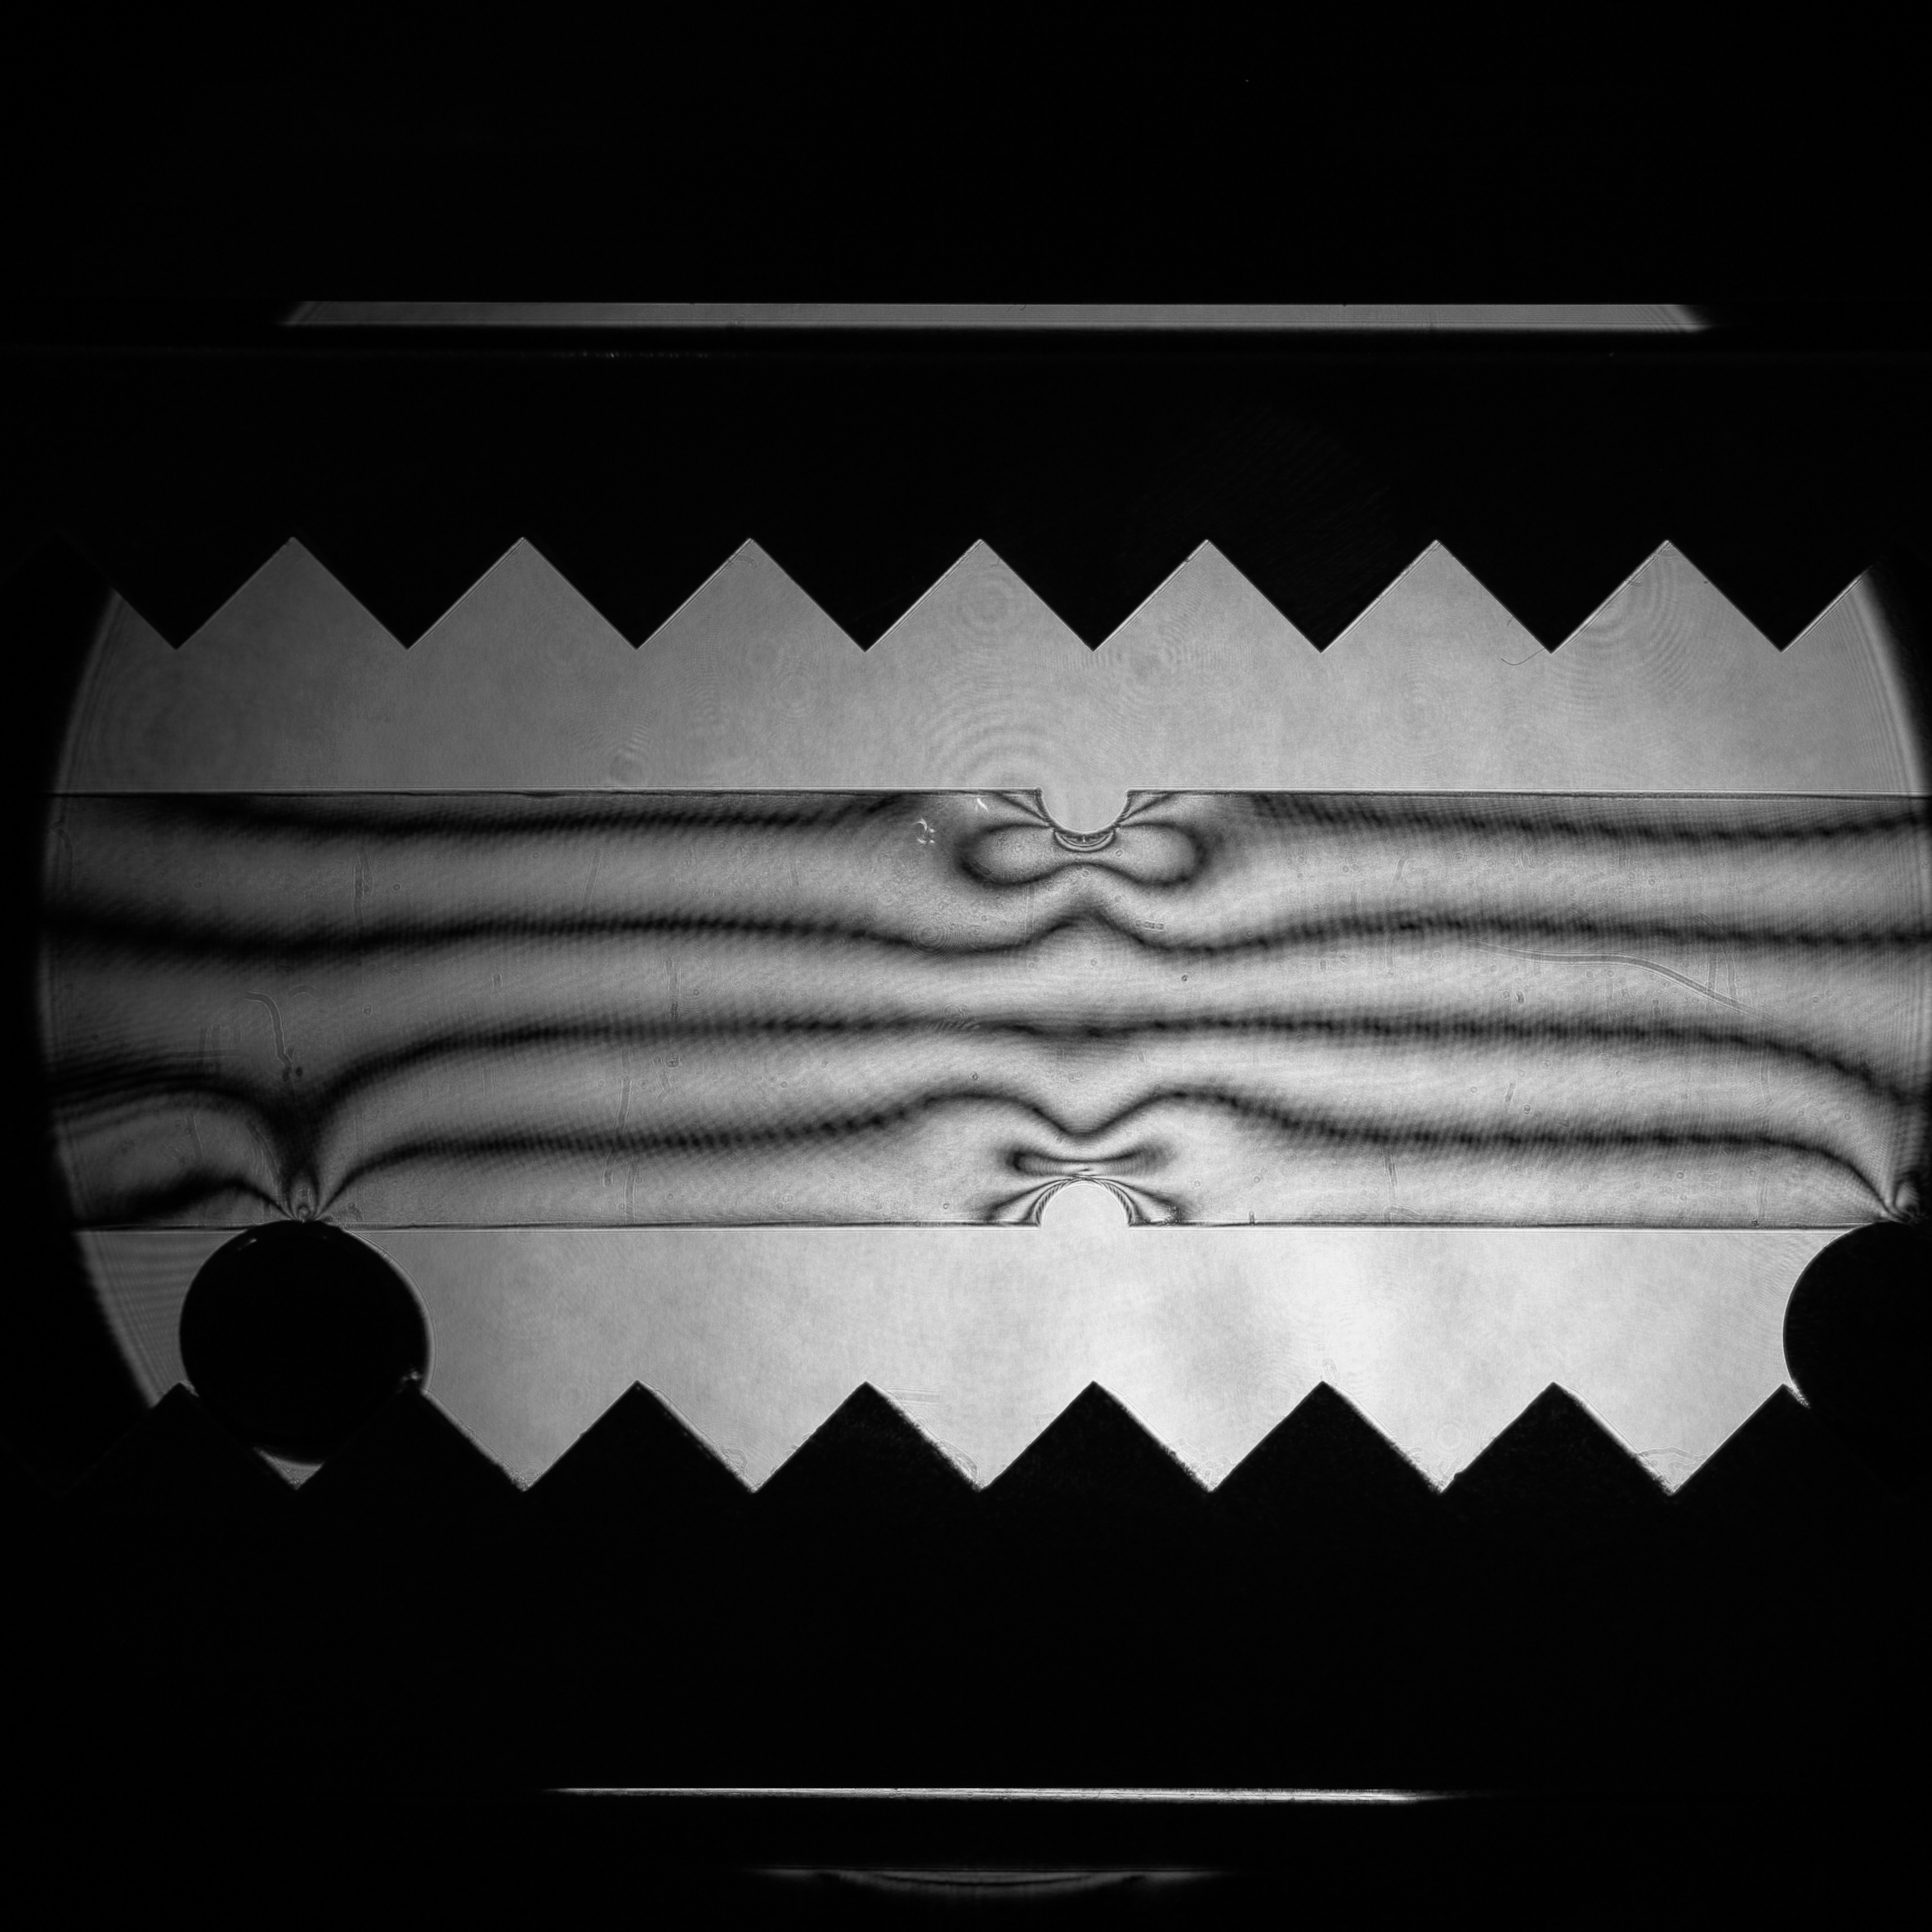
\includegraphics[width=\textwidth]{ρ=2.JPG}
        \caption{$\rho=2$}
    \end{minipage}
    \\ \vspace{5mm}
    \begin{minipage}[b]{0.48\textwidth}
        \centering
        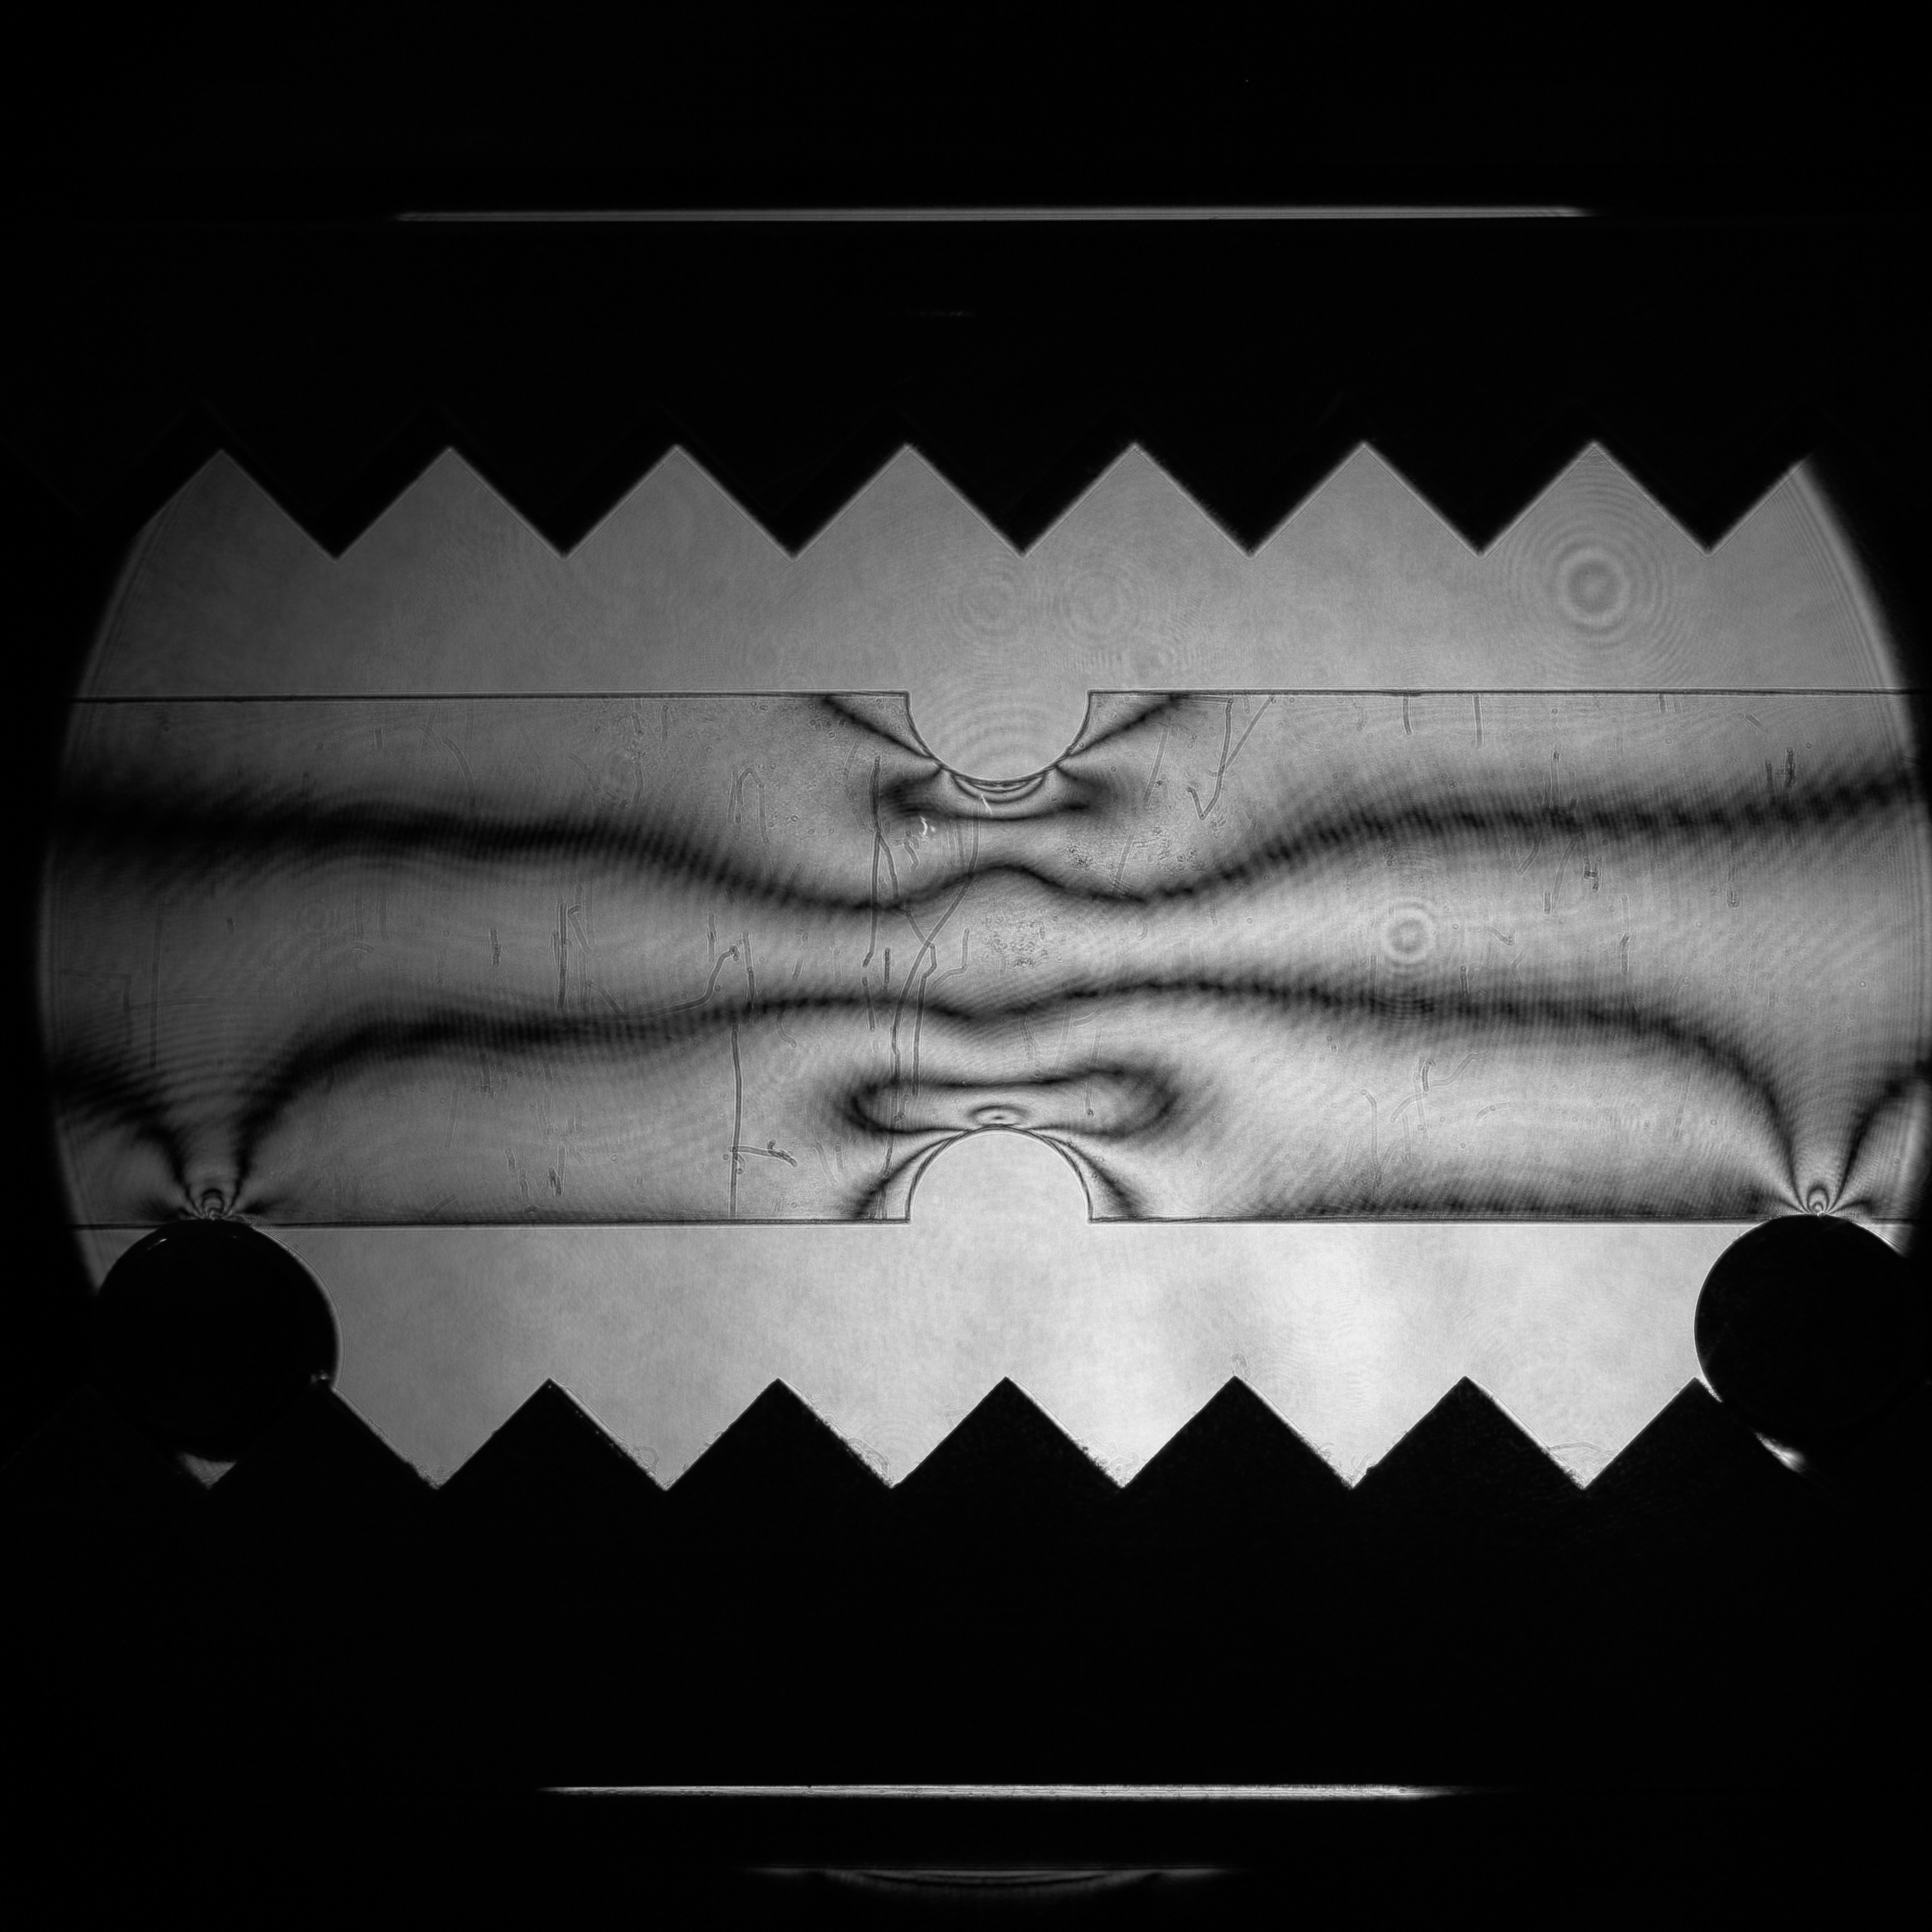
\includegraphics[width=\textwidth]{ρ=4.JPG}
        \caption{$\rho=4$}
    \end{minipage}
    \hfill
    \begin{minipage}[b]{0.48\textwidth}
        \centering
        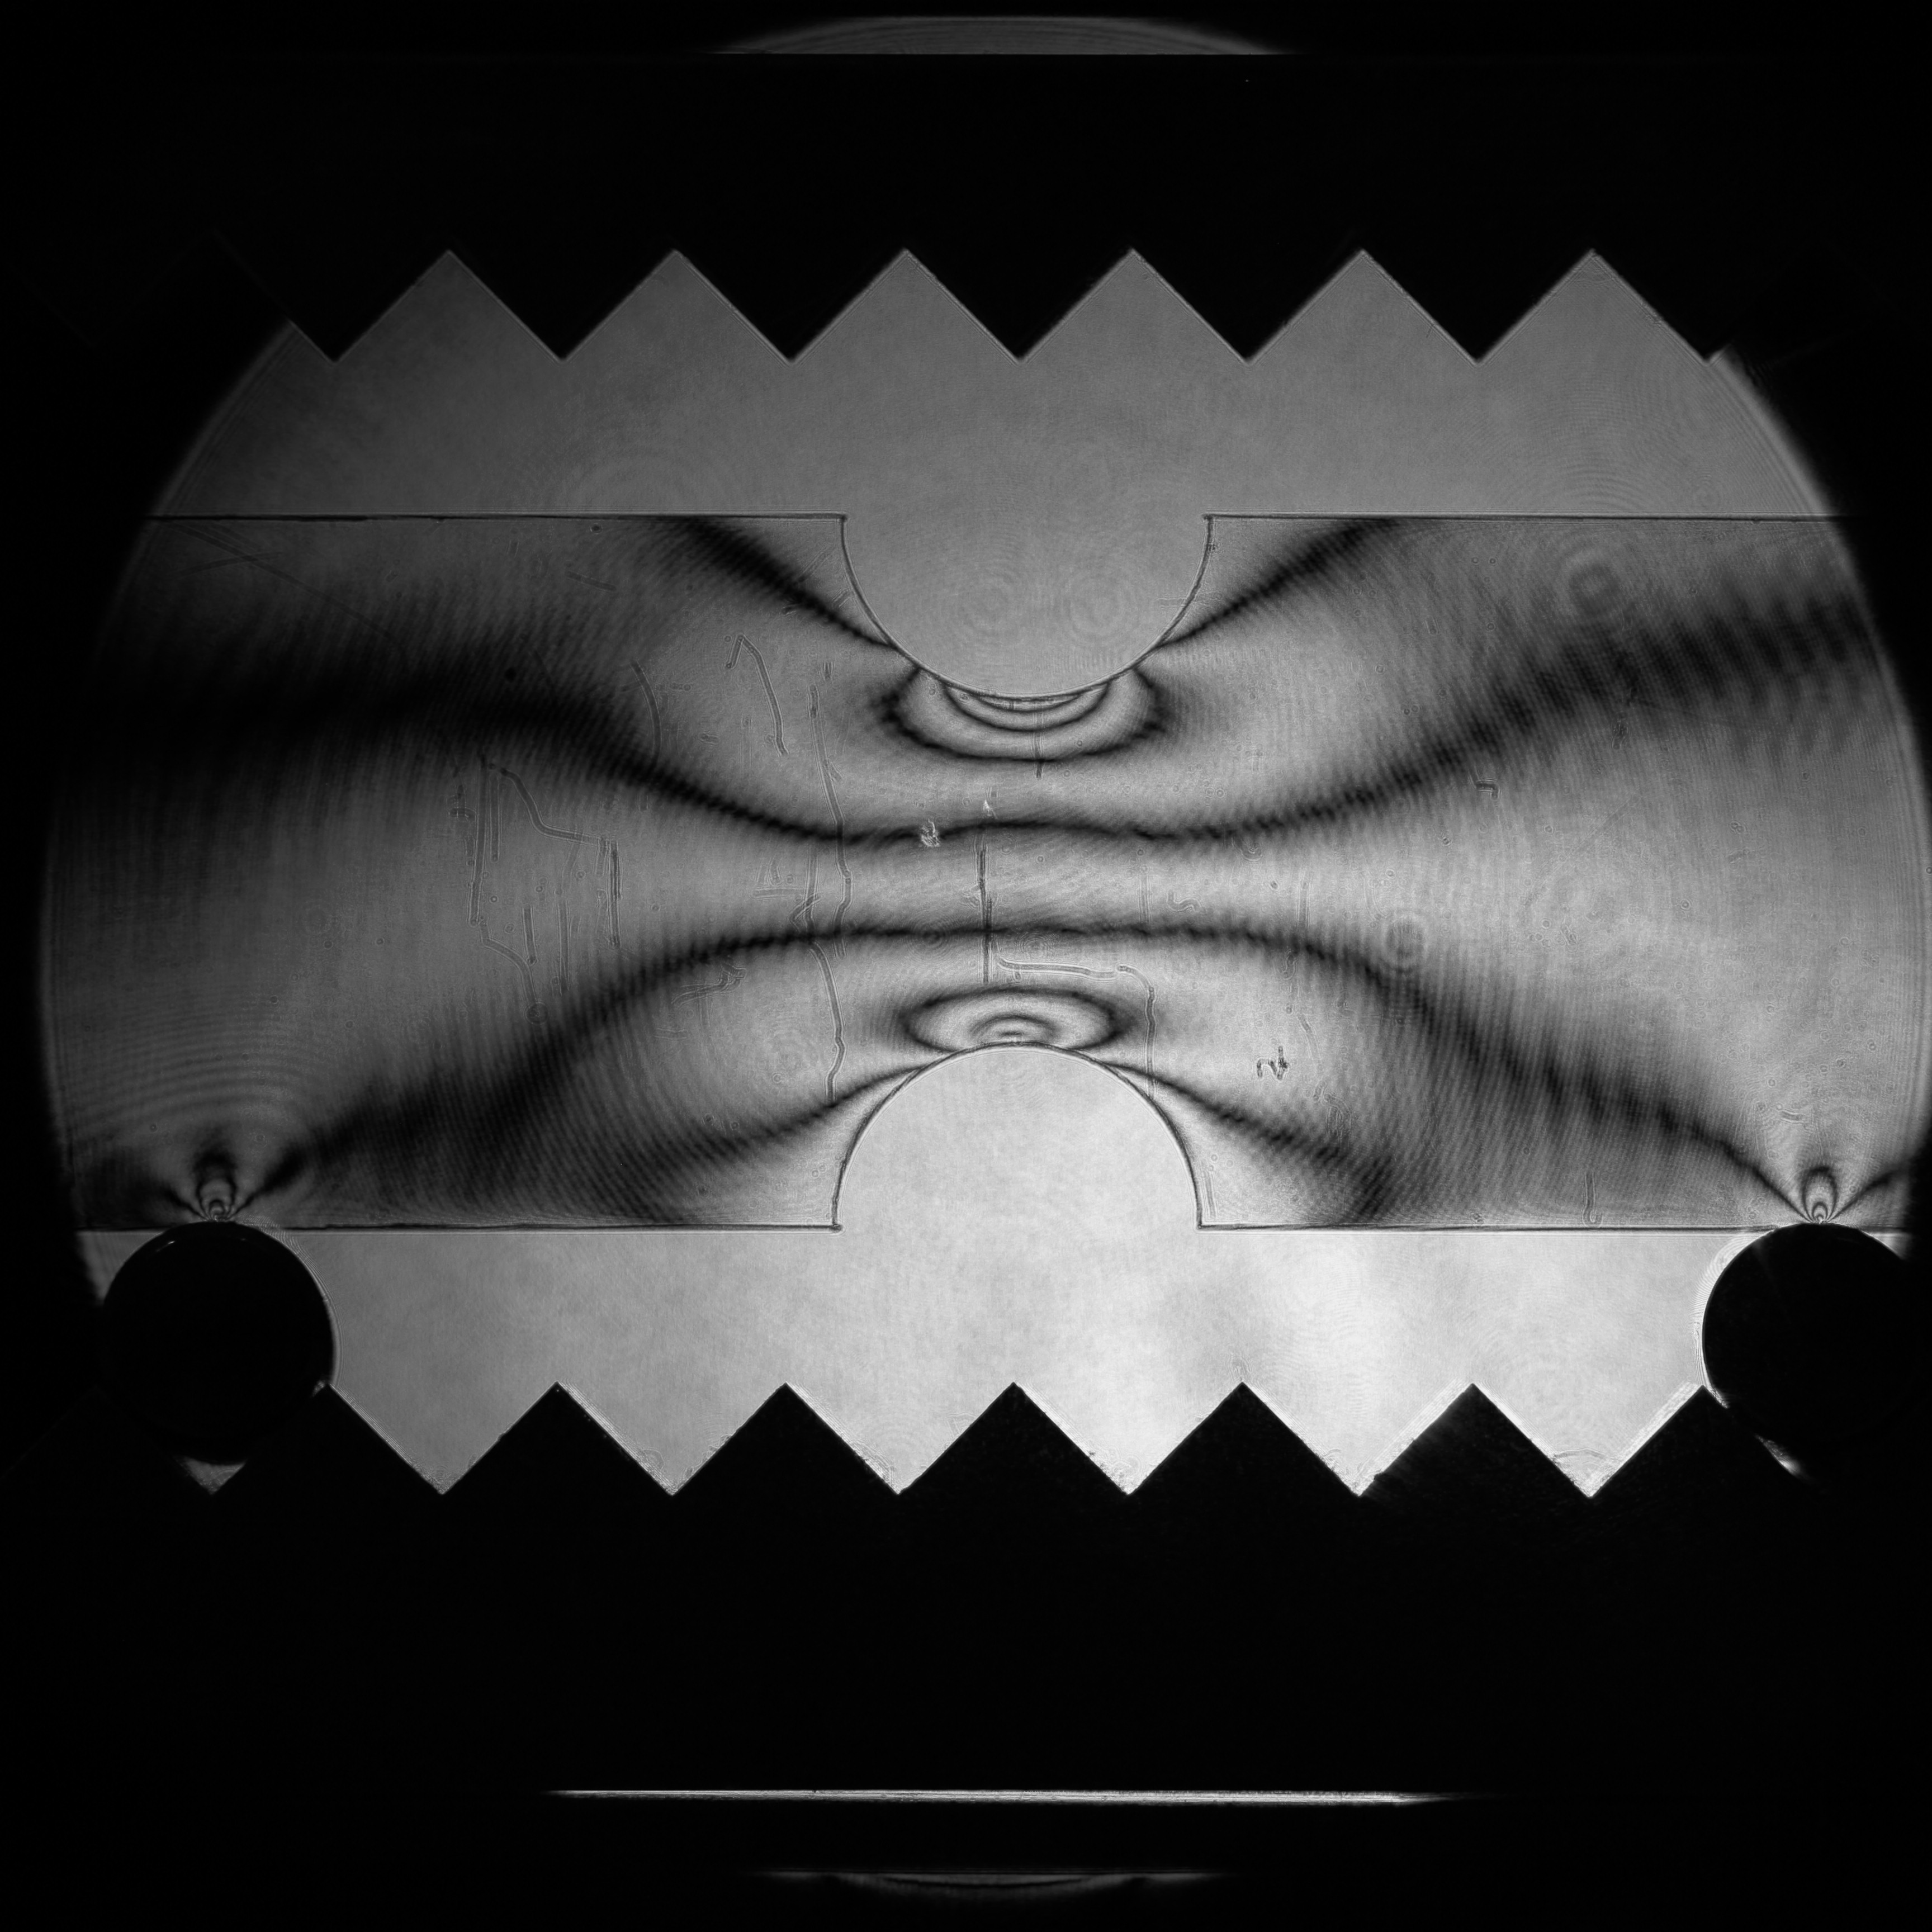
\includegraphics[width=\textwidth]{ρ=8.JPG}
        \caption{$\rho=8$}
    \end{minipage}
\end{figure}

このとき、応力集中係数$K$は以下の式で定義される。
\[
  K = \frac{\sigma_{x,p}}{\sigma_{x,\text{nom}}}
\]
テキスト(1-23)式$N_{\text{max}}=3CWe/\lambda h^2$を用いると、$K$の式は$N_{\text{max}}$の比を用いて以下のように表すことができる。
\[
  K = \frac{N_{\text{max(切り欠きあり)}}}{N_{\text{max(切り欠きなし)}}}
\]
% TO DO: σnomでどんなデータを使ったのか説明する

$K$(下限)と$K$(上限)の算出結果、およびPetersonの値との誤差は表3のようになった。

\begin{table}[H]
\centering
\caption{実験から求めた応力集中係数とPetersonの係数との比較}
\begin{tabular}{cccccc}
\hline
切欠き半径 $\rho$ (m) & $K$(上限) & $K$(下限) & $K_{\text{Peterson}}$ & 誤差(上限) [\%] & 誤差(下限) [\%] \\ \hline
$8.00 \times 10^{-3}$ & 1.52 & 1.42 & 1.33 & 14.59 & 6.60 \\
$4.00 \times 10^{-3}$ & 1.56 & 1.56 & 1.60 & 2.53  & 2.53 \\
$2.00 \times 10^{-3}$ & 1.95 & 1.91 & 2.00 & 2.53  & 4.30 \\
$1.00 \times 10^{-3}$ & 2.48 & 1.98 & 2.39 & 3.81  & 16.95 \\ \hline
\end{tabular}
\end{table}

この結果を下図のPetersonの応力集中係数と比較すると以下の図のようになる。
\begin{figure}[H]
    \centering
    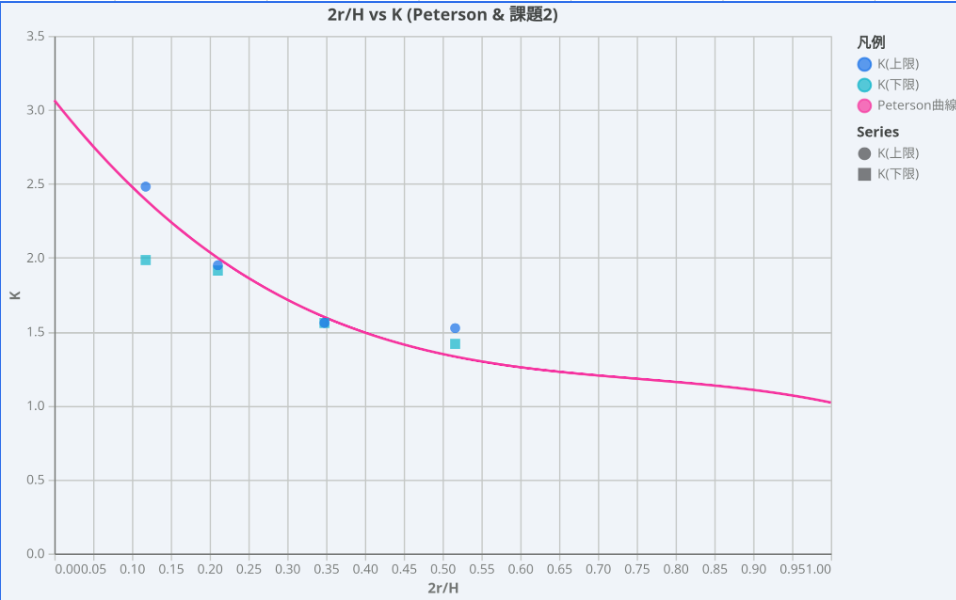
\includegraphics[width=10cm]{Peterson_compare.png}
    \caption{実験結果とPetersonの応力集中係数との比較}
\end{figure}

この図から、切り欠きの半径$\rho$が小さくなるほど応力集中係数$K$が大きくなることが今回の実験から確認できた。\\
一方で下限、上限ともに誤差が存在し、この実験の要因として以下のことが挙げられる。
\begin{itemize}
    \item 中心軸が梁の幾何学的中心ではなかったこと。
    \item 梁の切り欠きの境界においては縞が多く重なっており、正確に読み取ることが難しかったこと。
\end{itemize}
特に、梁の切り欠き境界における縞の重なりによって、$\rho=1$において大きな誤差が生まれたと考えられる。\\
また、今回の計算において$N_{\text{max(切り欠きなし)}}$は課題1の平均を用いているため、同様の値を用いているとすると相対誤差は
\[
  \frac{\Delta K}{K} = \frac{\Delta N_{\text{max}}}{N_{\text{max}}}
\]
となる。よって、$N_{\text{max}}$がより小さいもの、つまり$\rho$がより大きな条件において誤差が相対的に大きくなったと考えられる。

本実験における測定手法に関する課題として、以下のことが挙げられる。
\begin{itemize}
    \item 実験では縞模様の中心や数を主観的に判断したが、この縞次数の判別には客観的な基準が必要である。
    \item 4点の支持部分における摩擦の影響を取り除き、純粋な荷重のみが梁に加わるようにすること。
\end{itemize}
加えて、これらを改善すべき具体的な策として以下が挙げられる。
\begin{itemize}
    \item アプリケーション等を用いてピクセルの彩度などを解析することで、客観的な基準で縞次数を判別すること。
    \item 4点の支持部分に潤滑油をさすなどし、摩擦の影響を物理的に減らすこと。
\end{itemize}

\subsubsection*{課題3}
FreeCADの有限要素解析機能を用いて、両側半円欠き付き梁の応力解析を行った。
切り欠き半径$\rho=1$における応力分布は図13のようになった。
\begin{figure}[H]
    \centering
    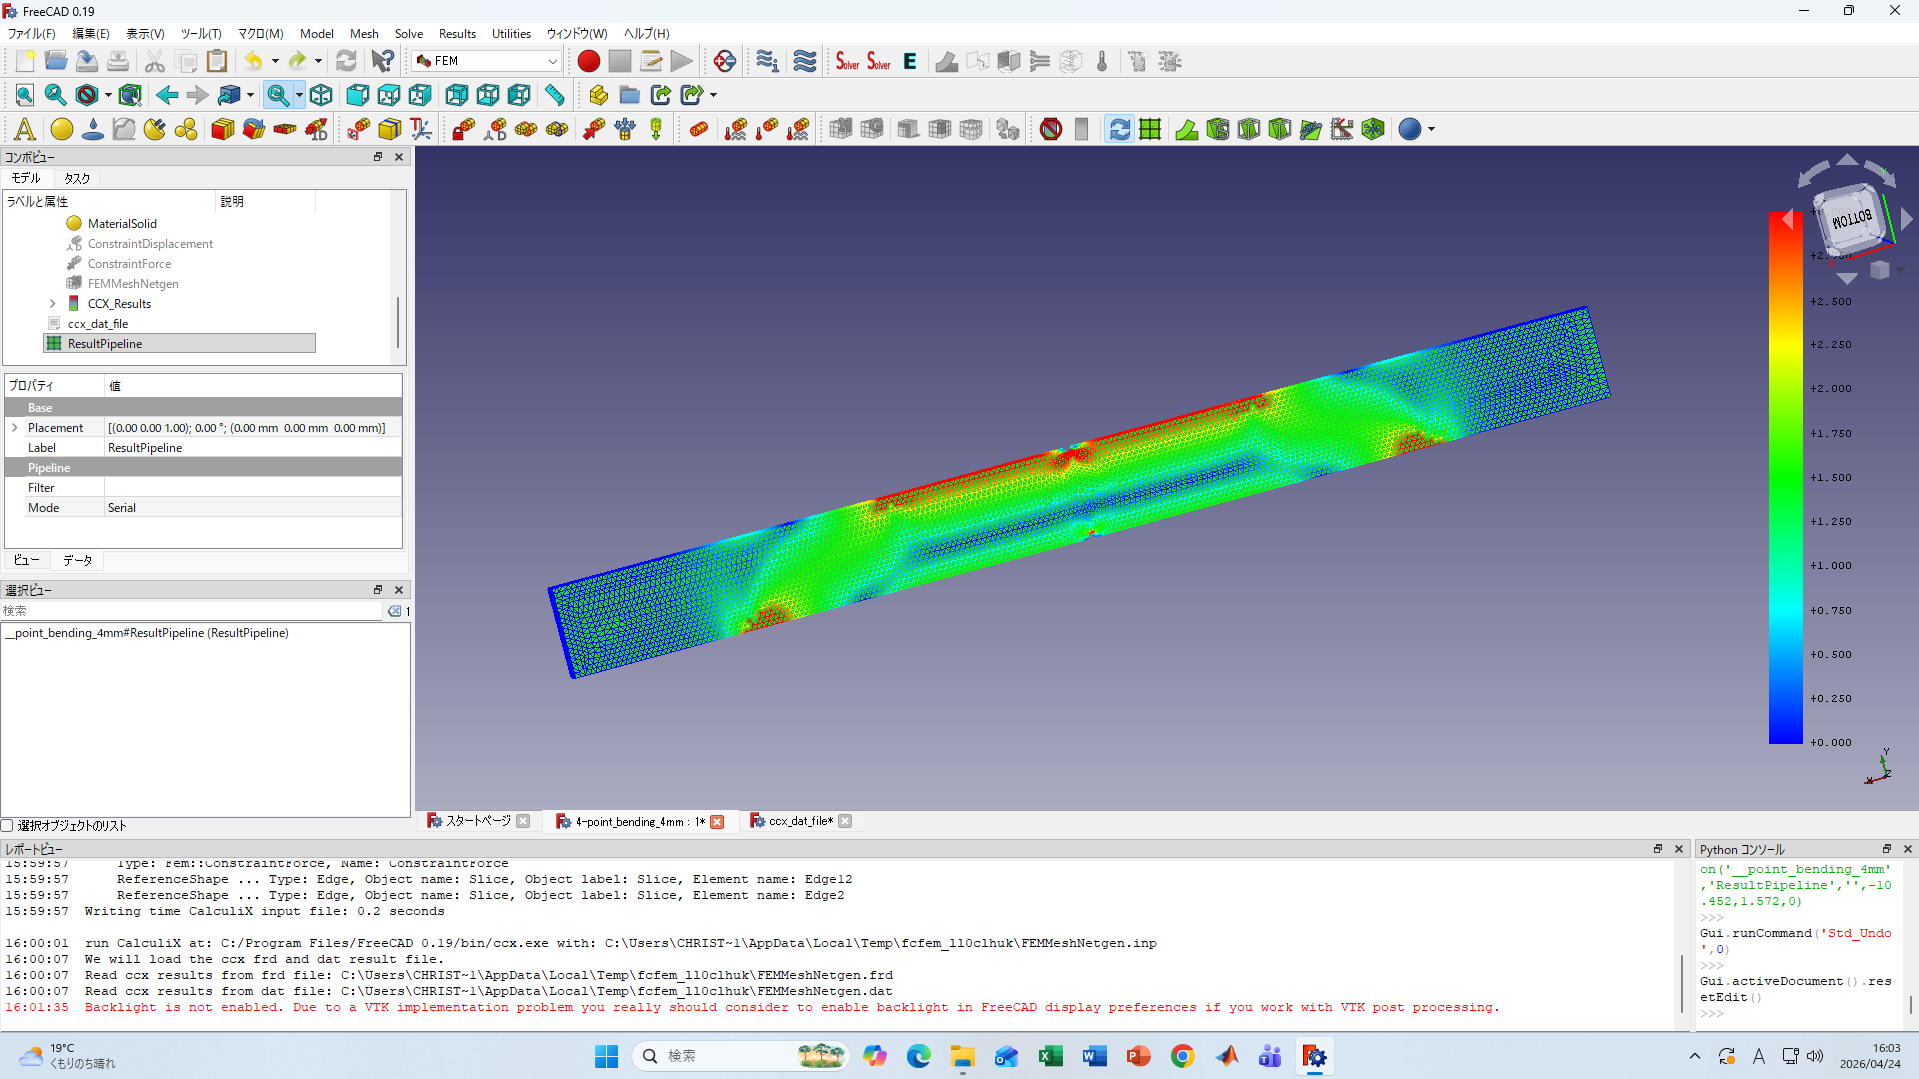
\includegraphics[width=10cm]{応力分布(ρ=1).png}
    \caption{$\rho=1$における全体応力分布}
\end{figure}

また、各切り欠き半径における応力分布のグラフは以下の図の通りである。
\begin{figure}[H]
    \centering
    \begin{minipage}[b]{0.48\textwidth}
        \centering
        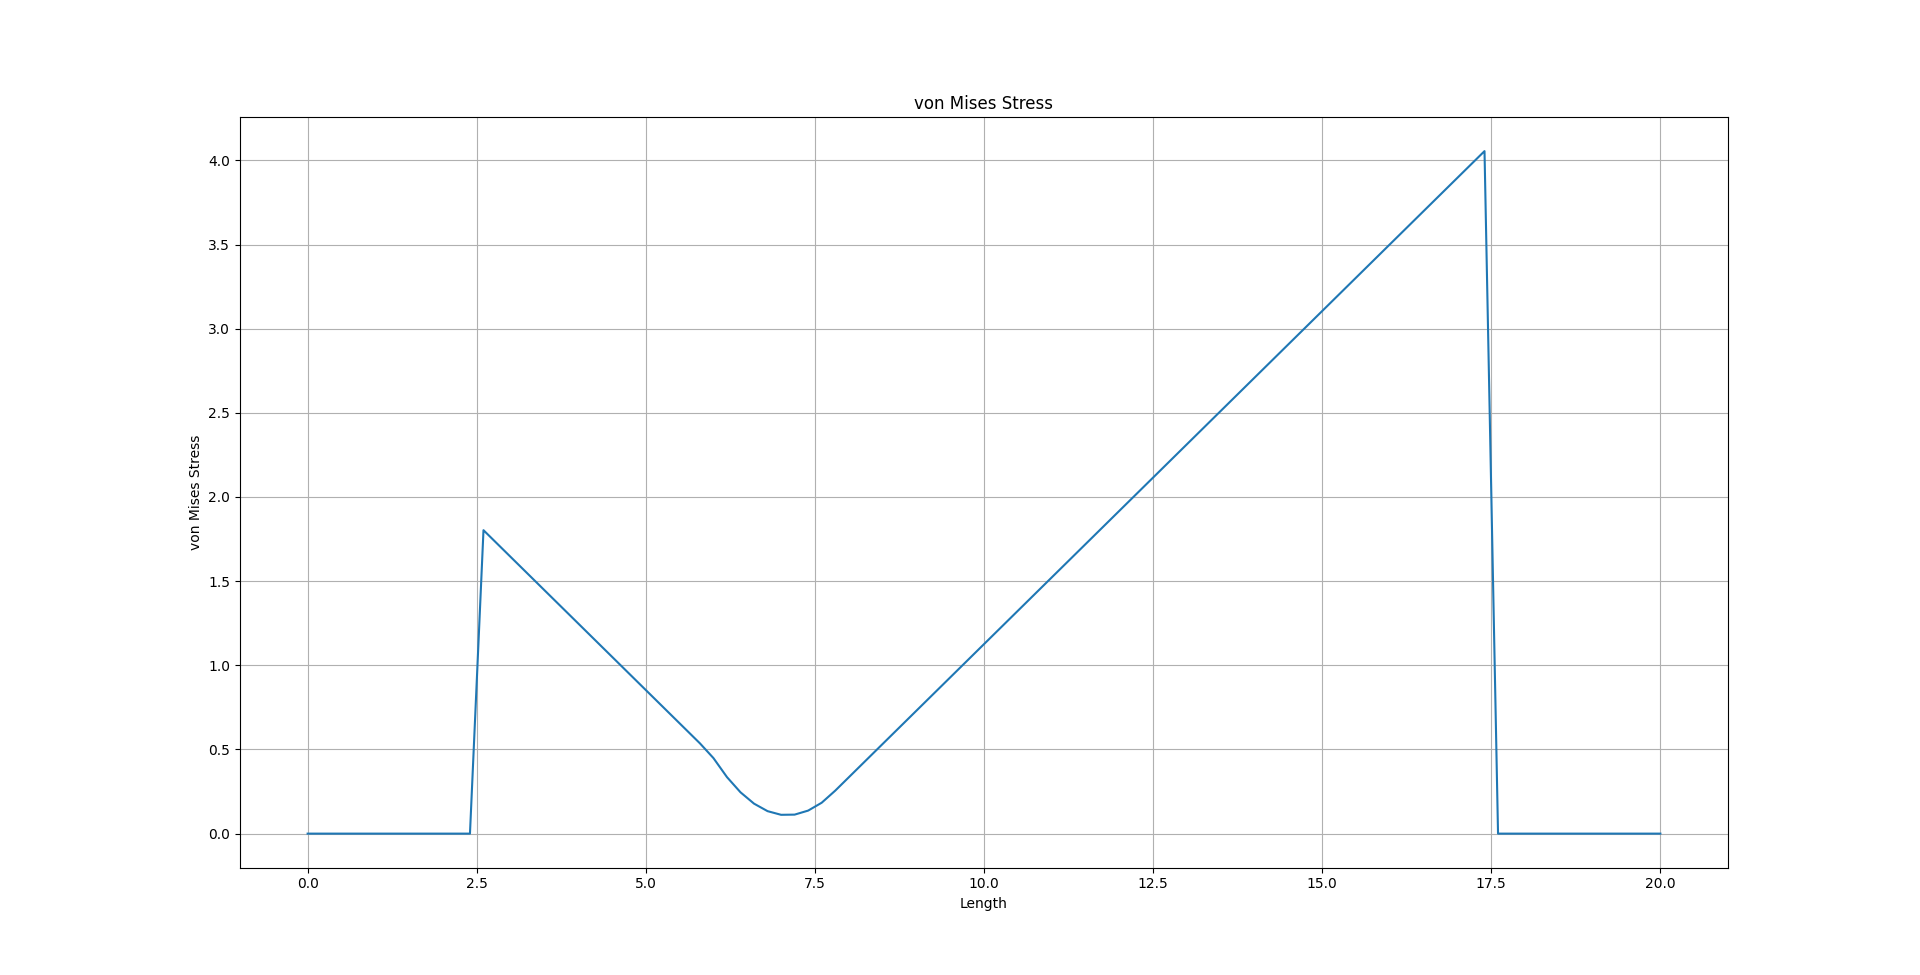
\includegraphics[width=\textwidth]{0mm_graph.png}
        \caption{切り欠きなしの応力分布}
    \end{minipage}
    \hfill
    \begin{minipage}[b]{0.48\textwidth}
        \centering
        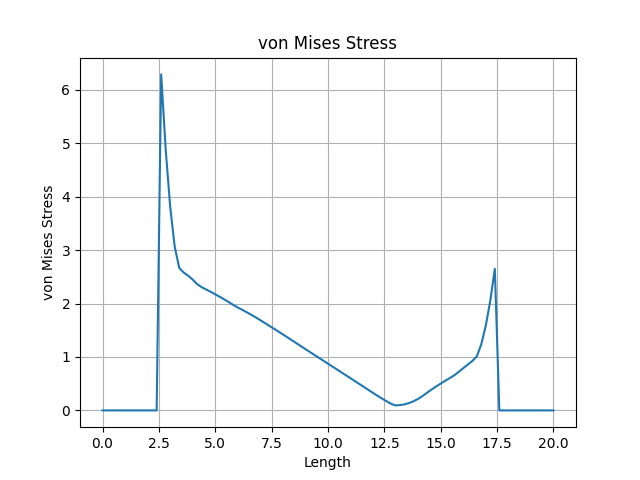
\includegraphics[width=\textwidth]{1mm_graph.png}
        \caption{$\rho=1$における応力分布}
    \end{minipage}
    \\ \vspace{5mm}
    \begin{minipage}[b]{0.48\textwidth}
        \centering
        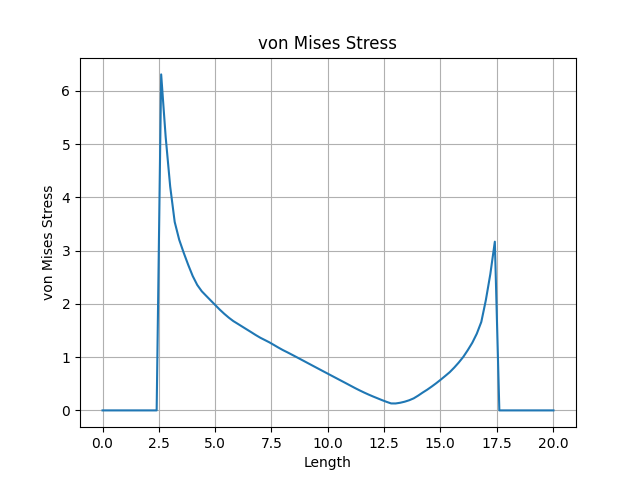
\includegraphics[width=\textwidth]{2mm_graph.png}
        \caption{$\rho=2$における応力分布}
    \end{minipage}
    \hfill
    \begin{minipage}[b]{0.48\textwidth}
        \centering
        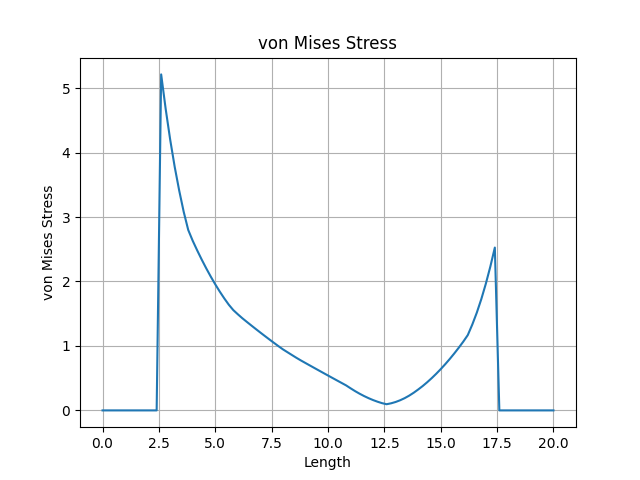
\includegraphics[width=\textwidth]{4mm_graph.png}
        \caption{$\rho=4$における応力分布}
    \end{minipage}
    \\ \vspace{5mm}
    \begin{minipage}[b]{0.48\textwidth}
        \centering
        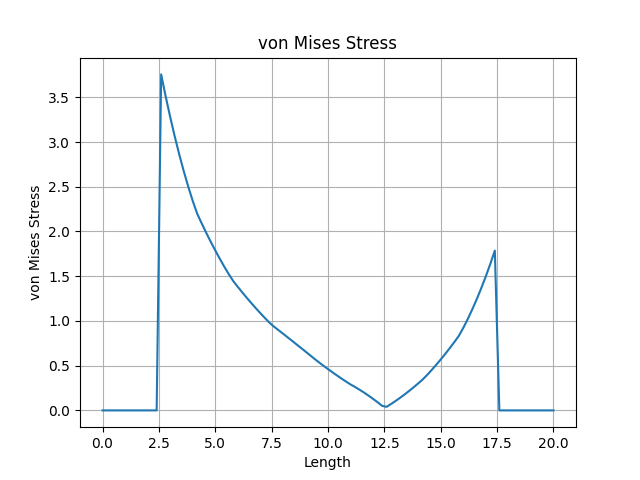
\includegraphics[width=\textwidth]{8mm_graph.png}
        \caption{$\rho=8$における応力分布}
    \end{minipage}
\end{figure}

この時、ピークの値を以下のように拡大して読み取った。この際、グラフの縦軸のラベルとしてvon Mises応力を用いた。
\begin{figure}[H]
    \centering
    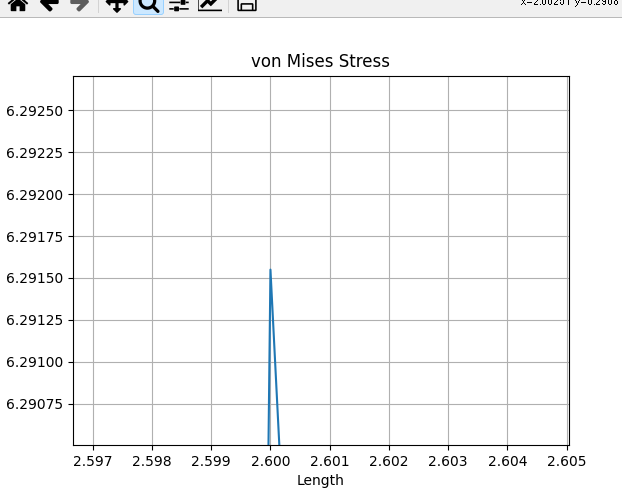
\includegraphics[width=8cm]{先端の値(ρ=1).png}
    \caption{$\rho=1$における先端値の拡大}
\end{figure}

ピークの値から求めた$K$値、課題2から求めた$K$値、およびPetersonの値の比較は表4のようになった。

\begin{table}[H]
\centering
\caption{各手法で得られた応力集中係数$K$の比較}
\begin{tabular}{cccc}
\hline
切欠き半径 $\rho$ (m) & $K$(課題2) & $K$(課題3) & $K_{\text{Peterson}}$ \\ \hline
$8.00 \times 10^{-3}$ & 1.52 & 1.39 & 1.33 \\
$4.00 \times 10^{-3}$ & 1.56 & 1.93 & 1.60 \\
$2.00 \times 10^{-3}$ & 1.95 & 2.34 & 2.00 \\
$1.00 \times 10^{-3}$ & 2.48 & 2.33 & 2.39 \\ \hline
\end{tabular}
\end{table}

以下が作成した解析モデルのメッシュ画像である。
\begin{figure}[H]
    \centering
    \begin{minipage}[b]{0.32\textwidth}
        \centering
        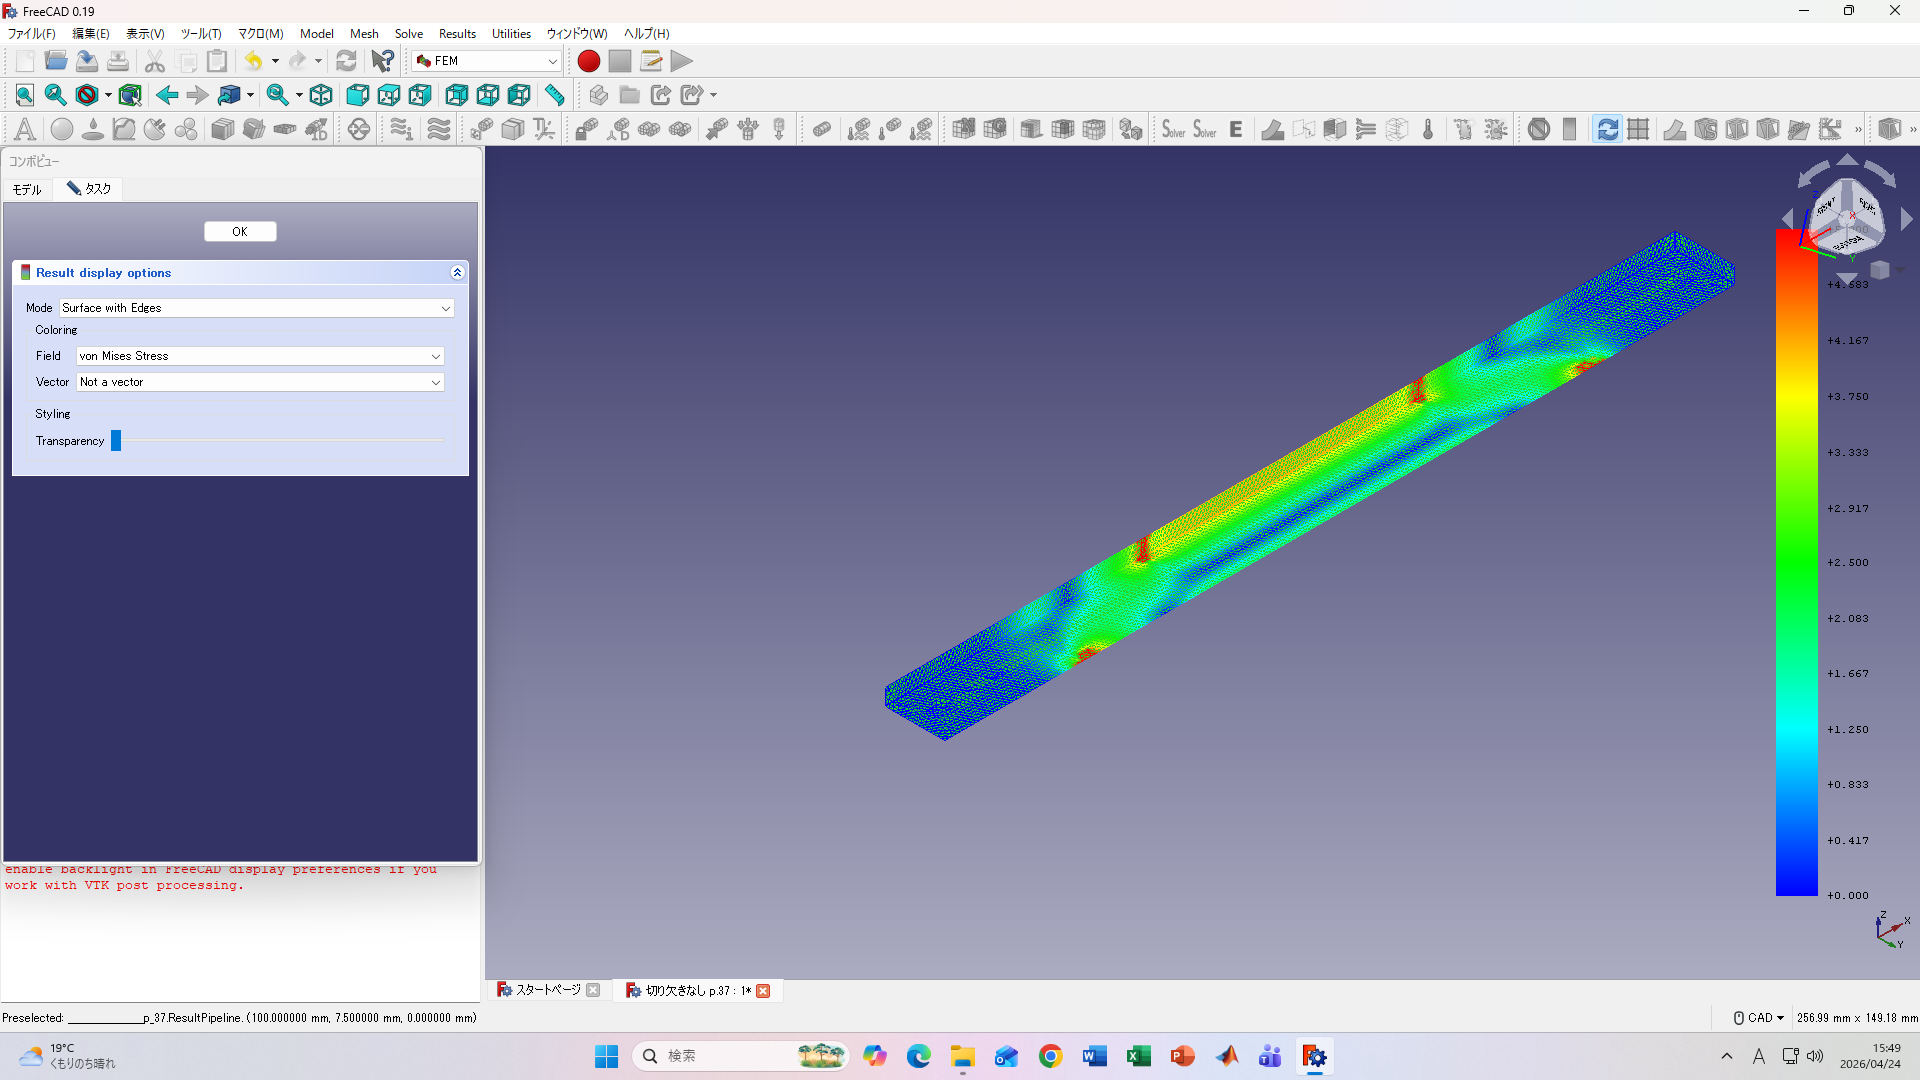
\includegraphics[width=\textwidth]{メッシュ_0mm.png}
        \caption{メッシュ(なし)}
    \end{minipage}
    \hfill
    \begin{minipage}[b]{0.32\textwidth}
        \centering
        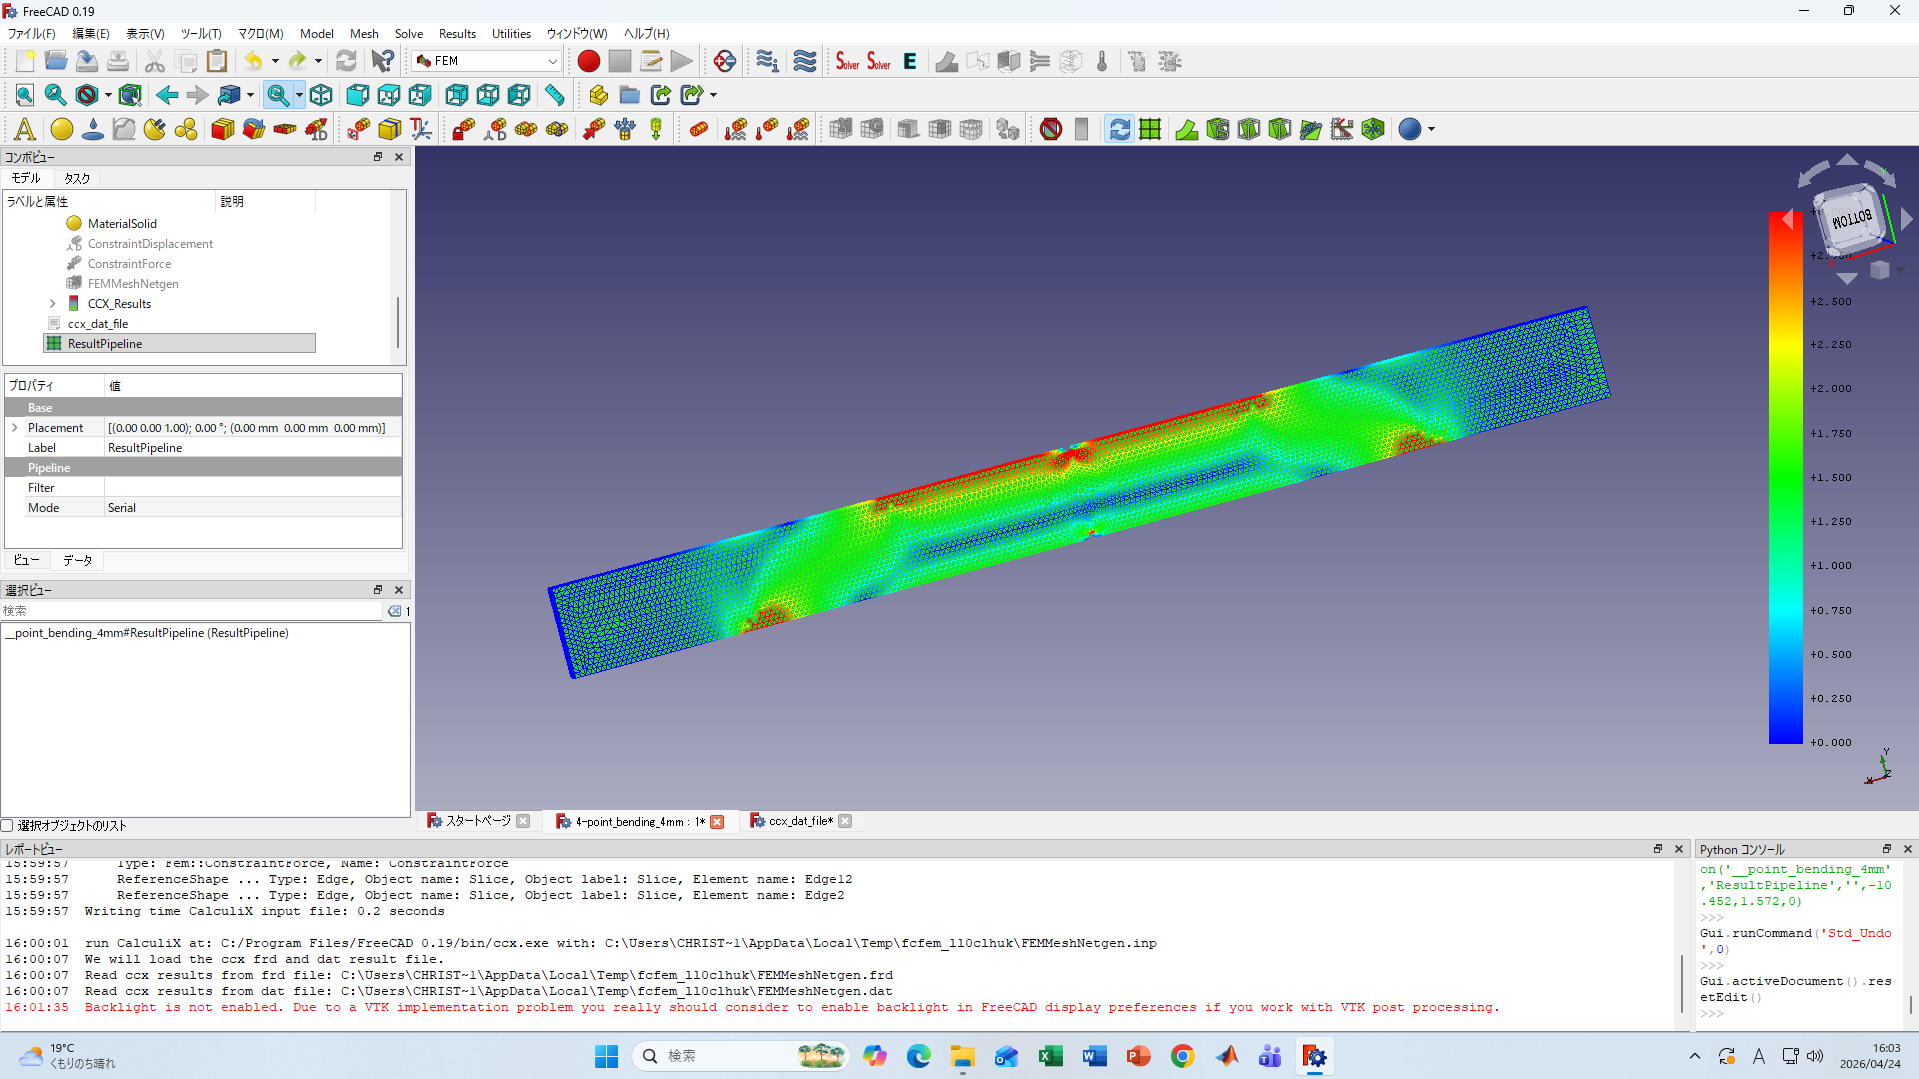
\includegraphics[width=\textwidth]{メッシュ_1mm.png}
        \caption{メッシュ($\rho=1$)}
    \end{minipage}
    \hfill
    \begin{minipage}[b]{0.32\textwidth}
        \centering
        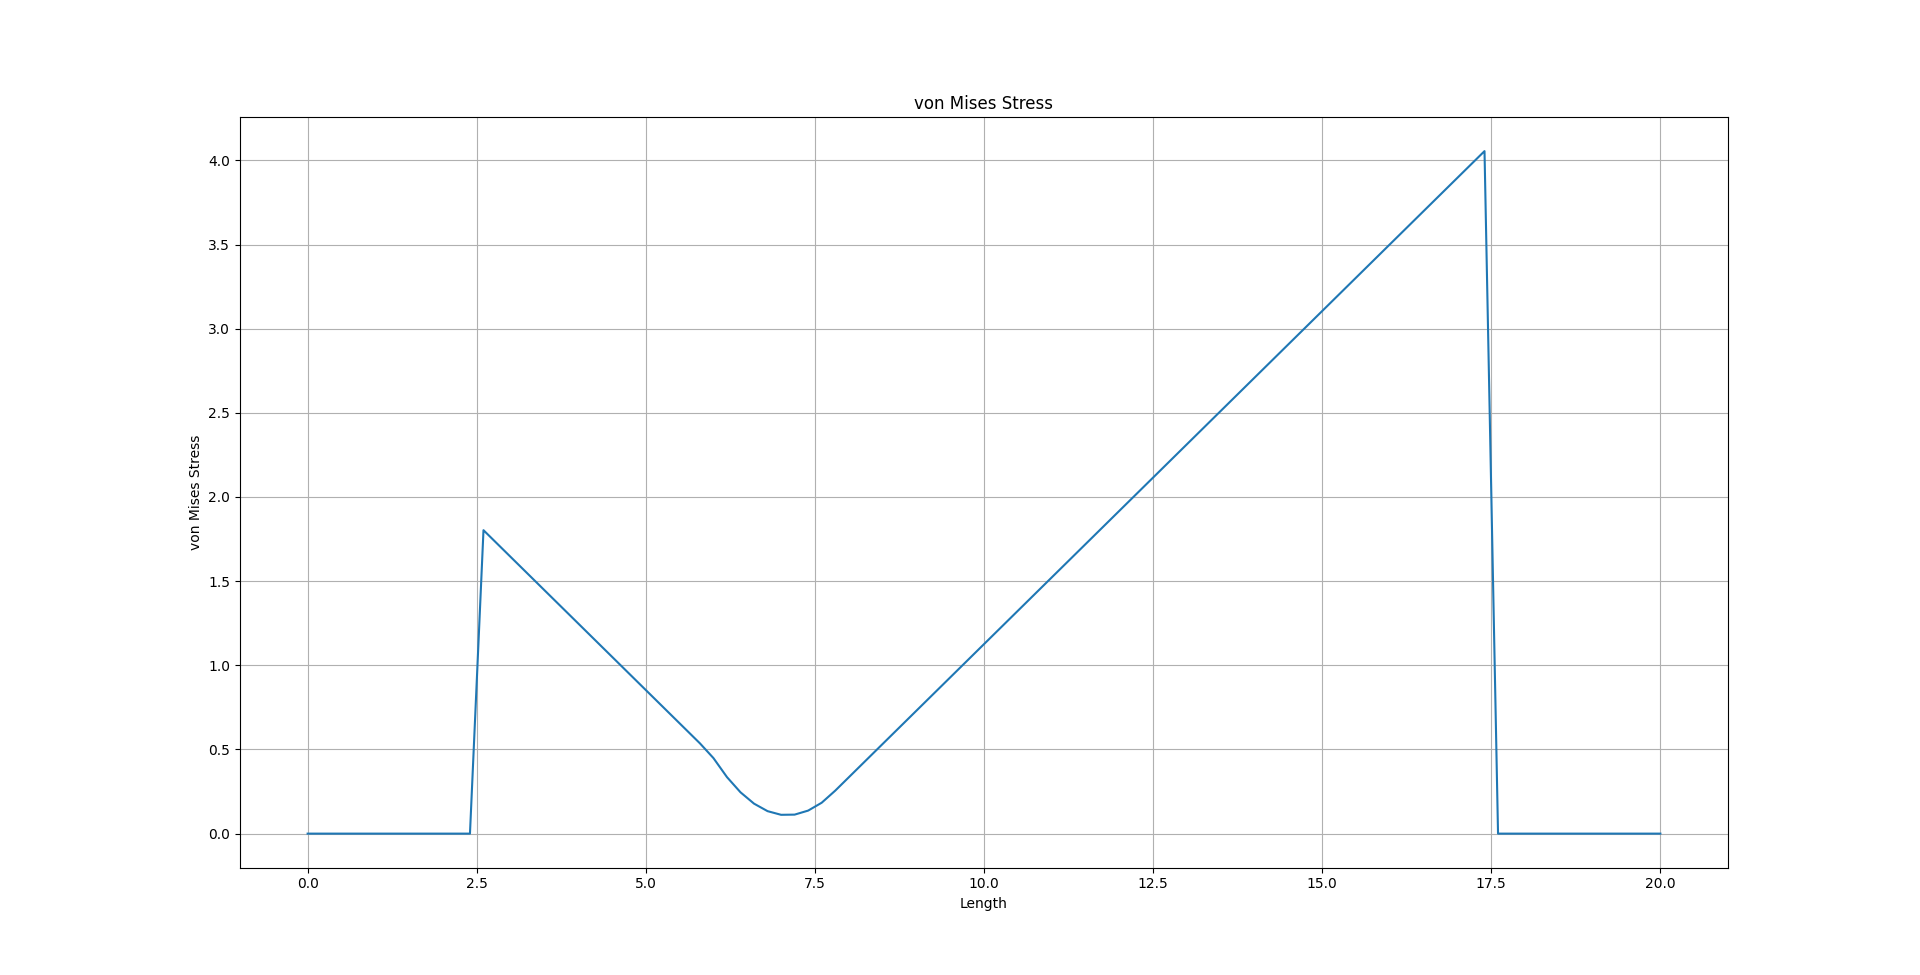
\includegraphics[width=\textwidth]{メッシュ_2mm.png}
        \caption{メッシュ($\rho=2$)}
    \end{minipage}
    \\ \vspace{5mm}
    \begin{minipage}[b]{0.48\textwidth}
        \centering
        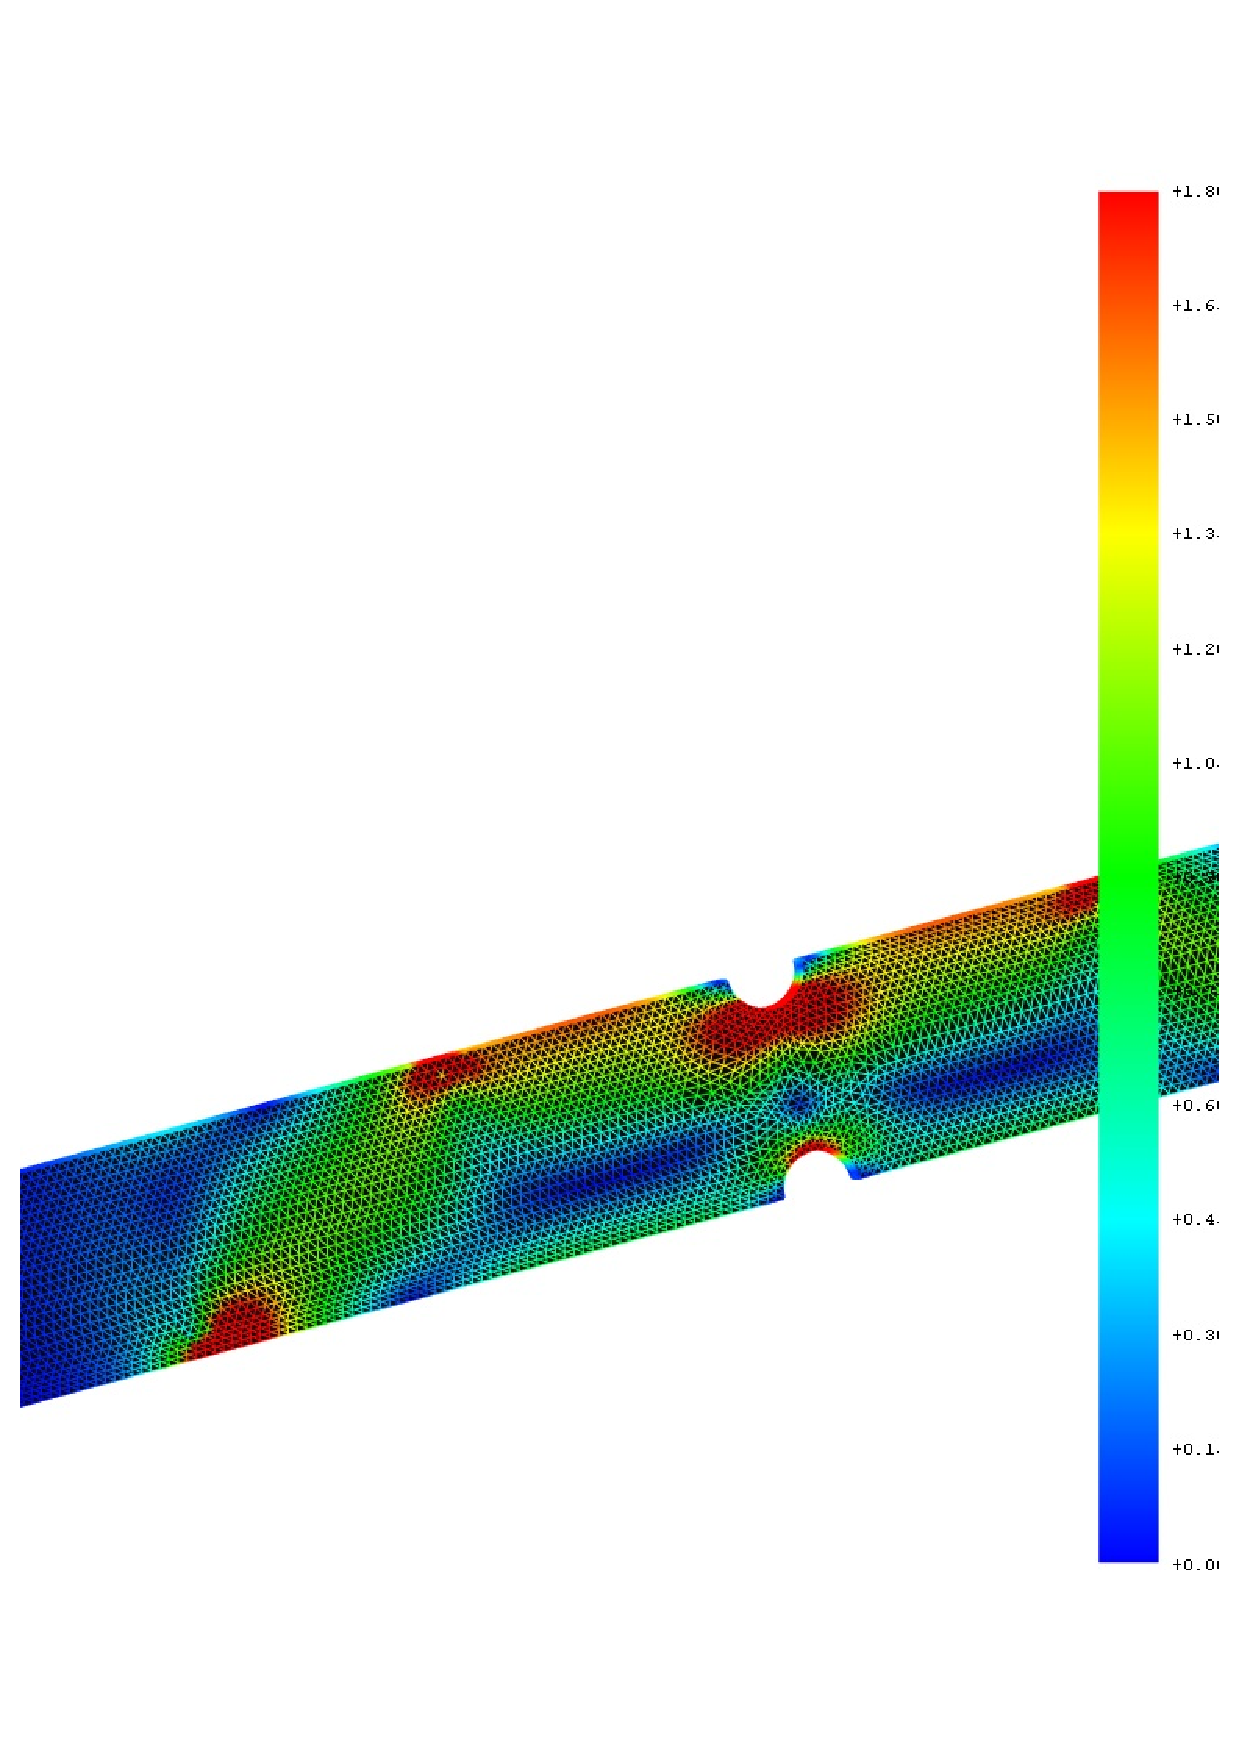
\includegraphics[width=\textwidth]{メッシュ_4mm.pdf}
        \caption{メッシュ($\rho=4$)}
    \end{minipage}
    \hfill
    \begin{minipage}[b]{0.48\textwidth}
        \centering
        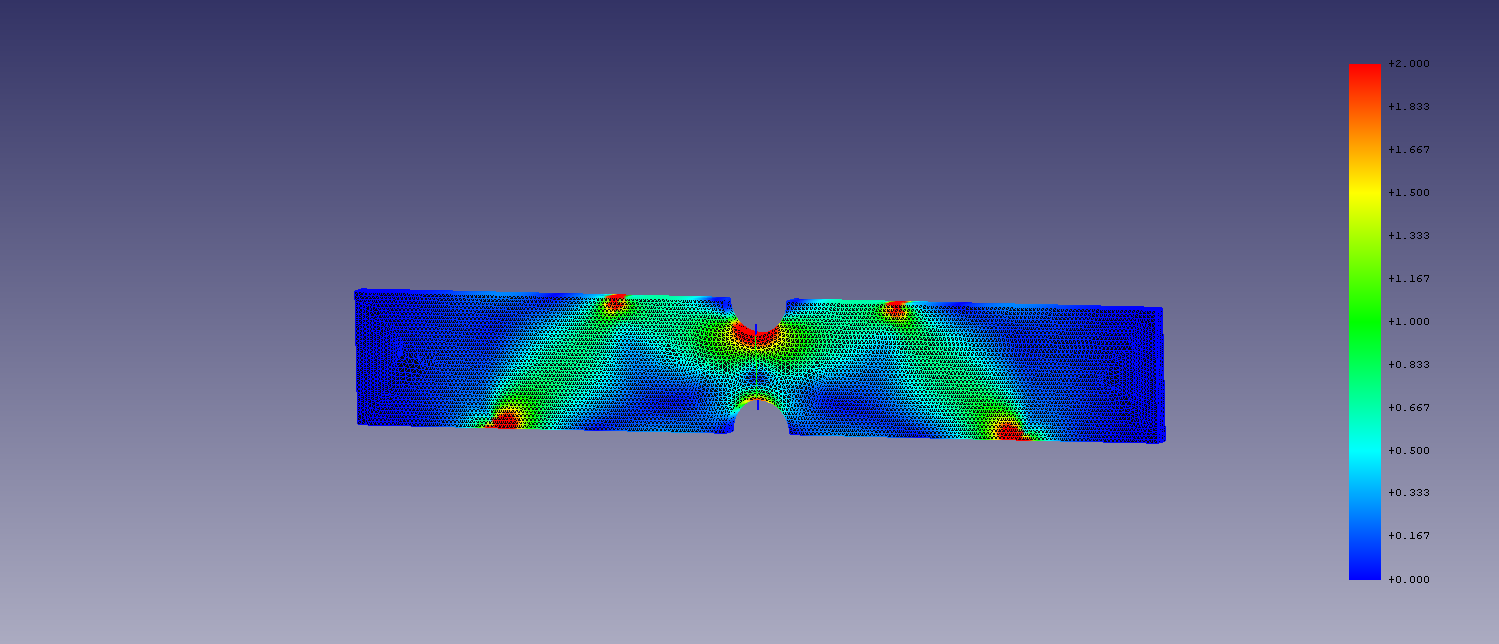
\includegraphics[width=\textwidth]{メッシュ_8mm.png}
        \caption{メッシュ($\rho=8$)}
    \end{minipage}
\end{figure}

まず、メッシュ作成時の要素の細かさが結果に及ぼす影響を考察する。\\
以下は切り欠きなしの梁に応力を加えた際の、メッシュが「中程度」のものと「細かい」ものの比較図である。
\begin{figure}[H]
    \centering
    \begin{minipage}[b]{0.48\textwidth}
        \centering
        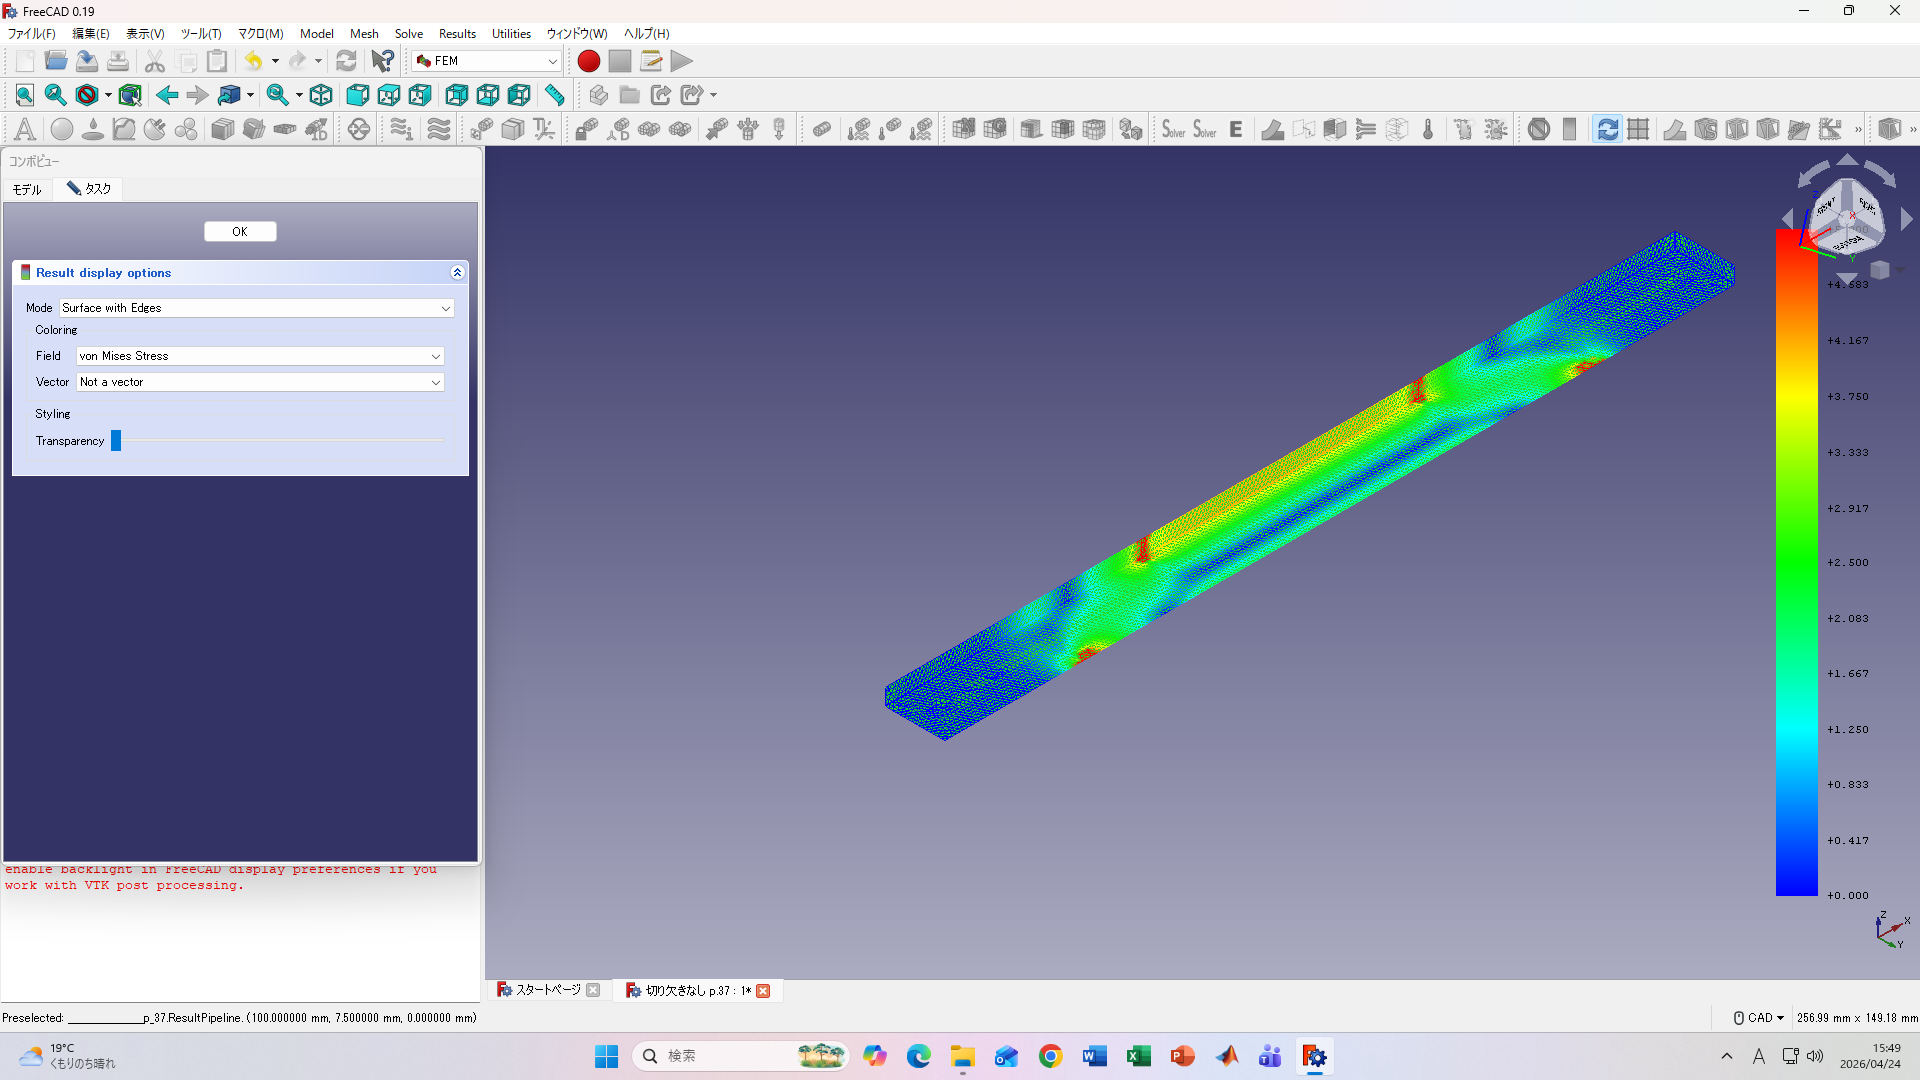
\includegraphics[width=\textwidth]{メッシュ中程度.png}
        \caption{メッシュ（中程度）の応力分布}
    \end{minipage}
    \hfill
    \begin{minipage}[b]{0.48\textwidth}
        \centering
        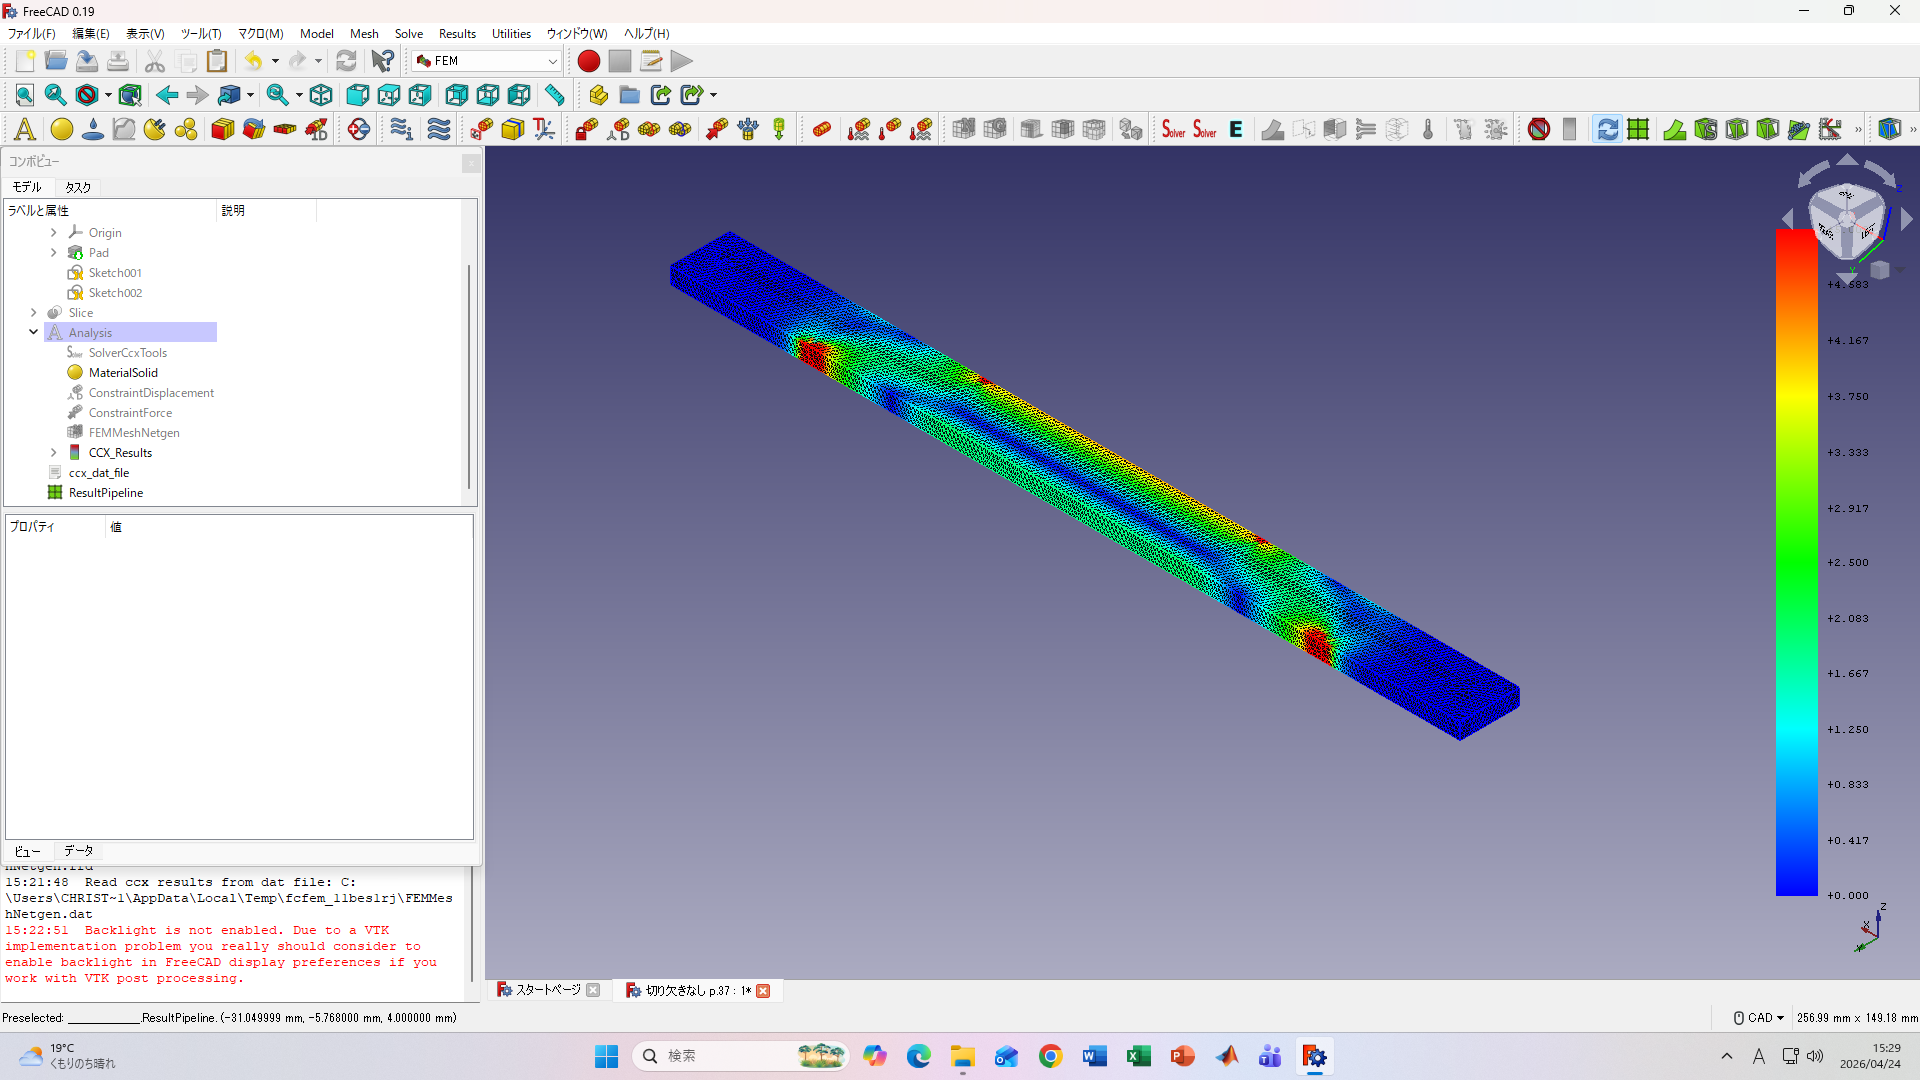
\includegraphics[width=\textwidth]{メッシュ細かい.png}
        \caption{メッシュ（細かい）の応力分布}
    \end{minipage}
\end{figure}

メッシュが細かいものについては、応力が最大となる4点の支点部分がより赤く表示され、ピークが鮮明に表されていることが分かる。一方で、中程度のメッシュのものでは最大応力がぼやけて分散されていることが分かる。これは、メッシュを大きく設定することで、応力がより大きなグリッド内で平均化されてしまうために起こると考えられる。\\
これにより、メッシュを大きくするにつれて有限要素解析によって求められる最大応力が小さく見積もられてしまい、結果としてより小さい$K$の値が算出されてしまうと考えられる。

% TO DO: いま課題3におけるKの値と近似によって求められるKの値を再びのせると以下のようになる。
% （ここに表やデータを追記）

次に、課題3で得られた梁の応力分布を、課題2における縞模様の実験結果と比較する。\\
$\rho=1$における課題2の光弾性画像と、課題3における有限要素法によって出力した画像を並べると以下のようになる。

\begin{figure}[H]
    \centering
    \begin{minipage}[b]{0.48\textwidth}
        \centering
        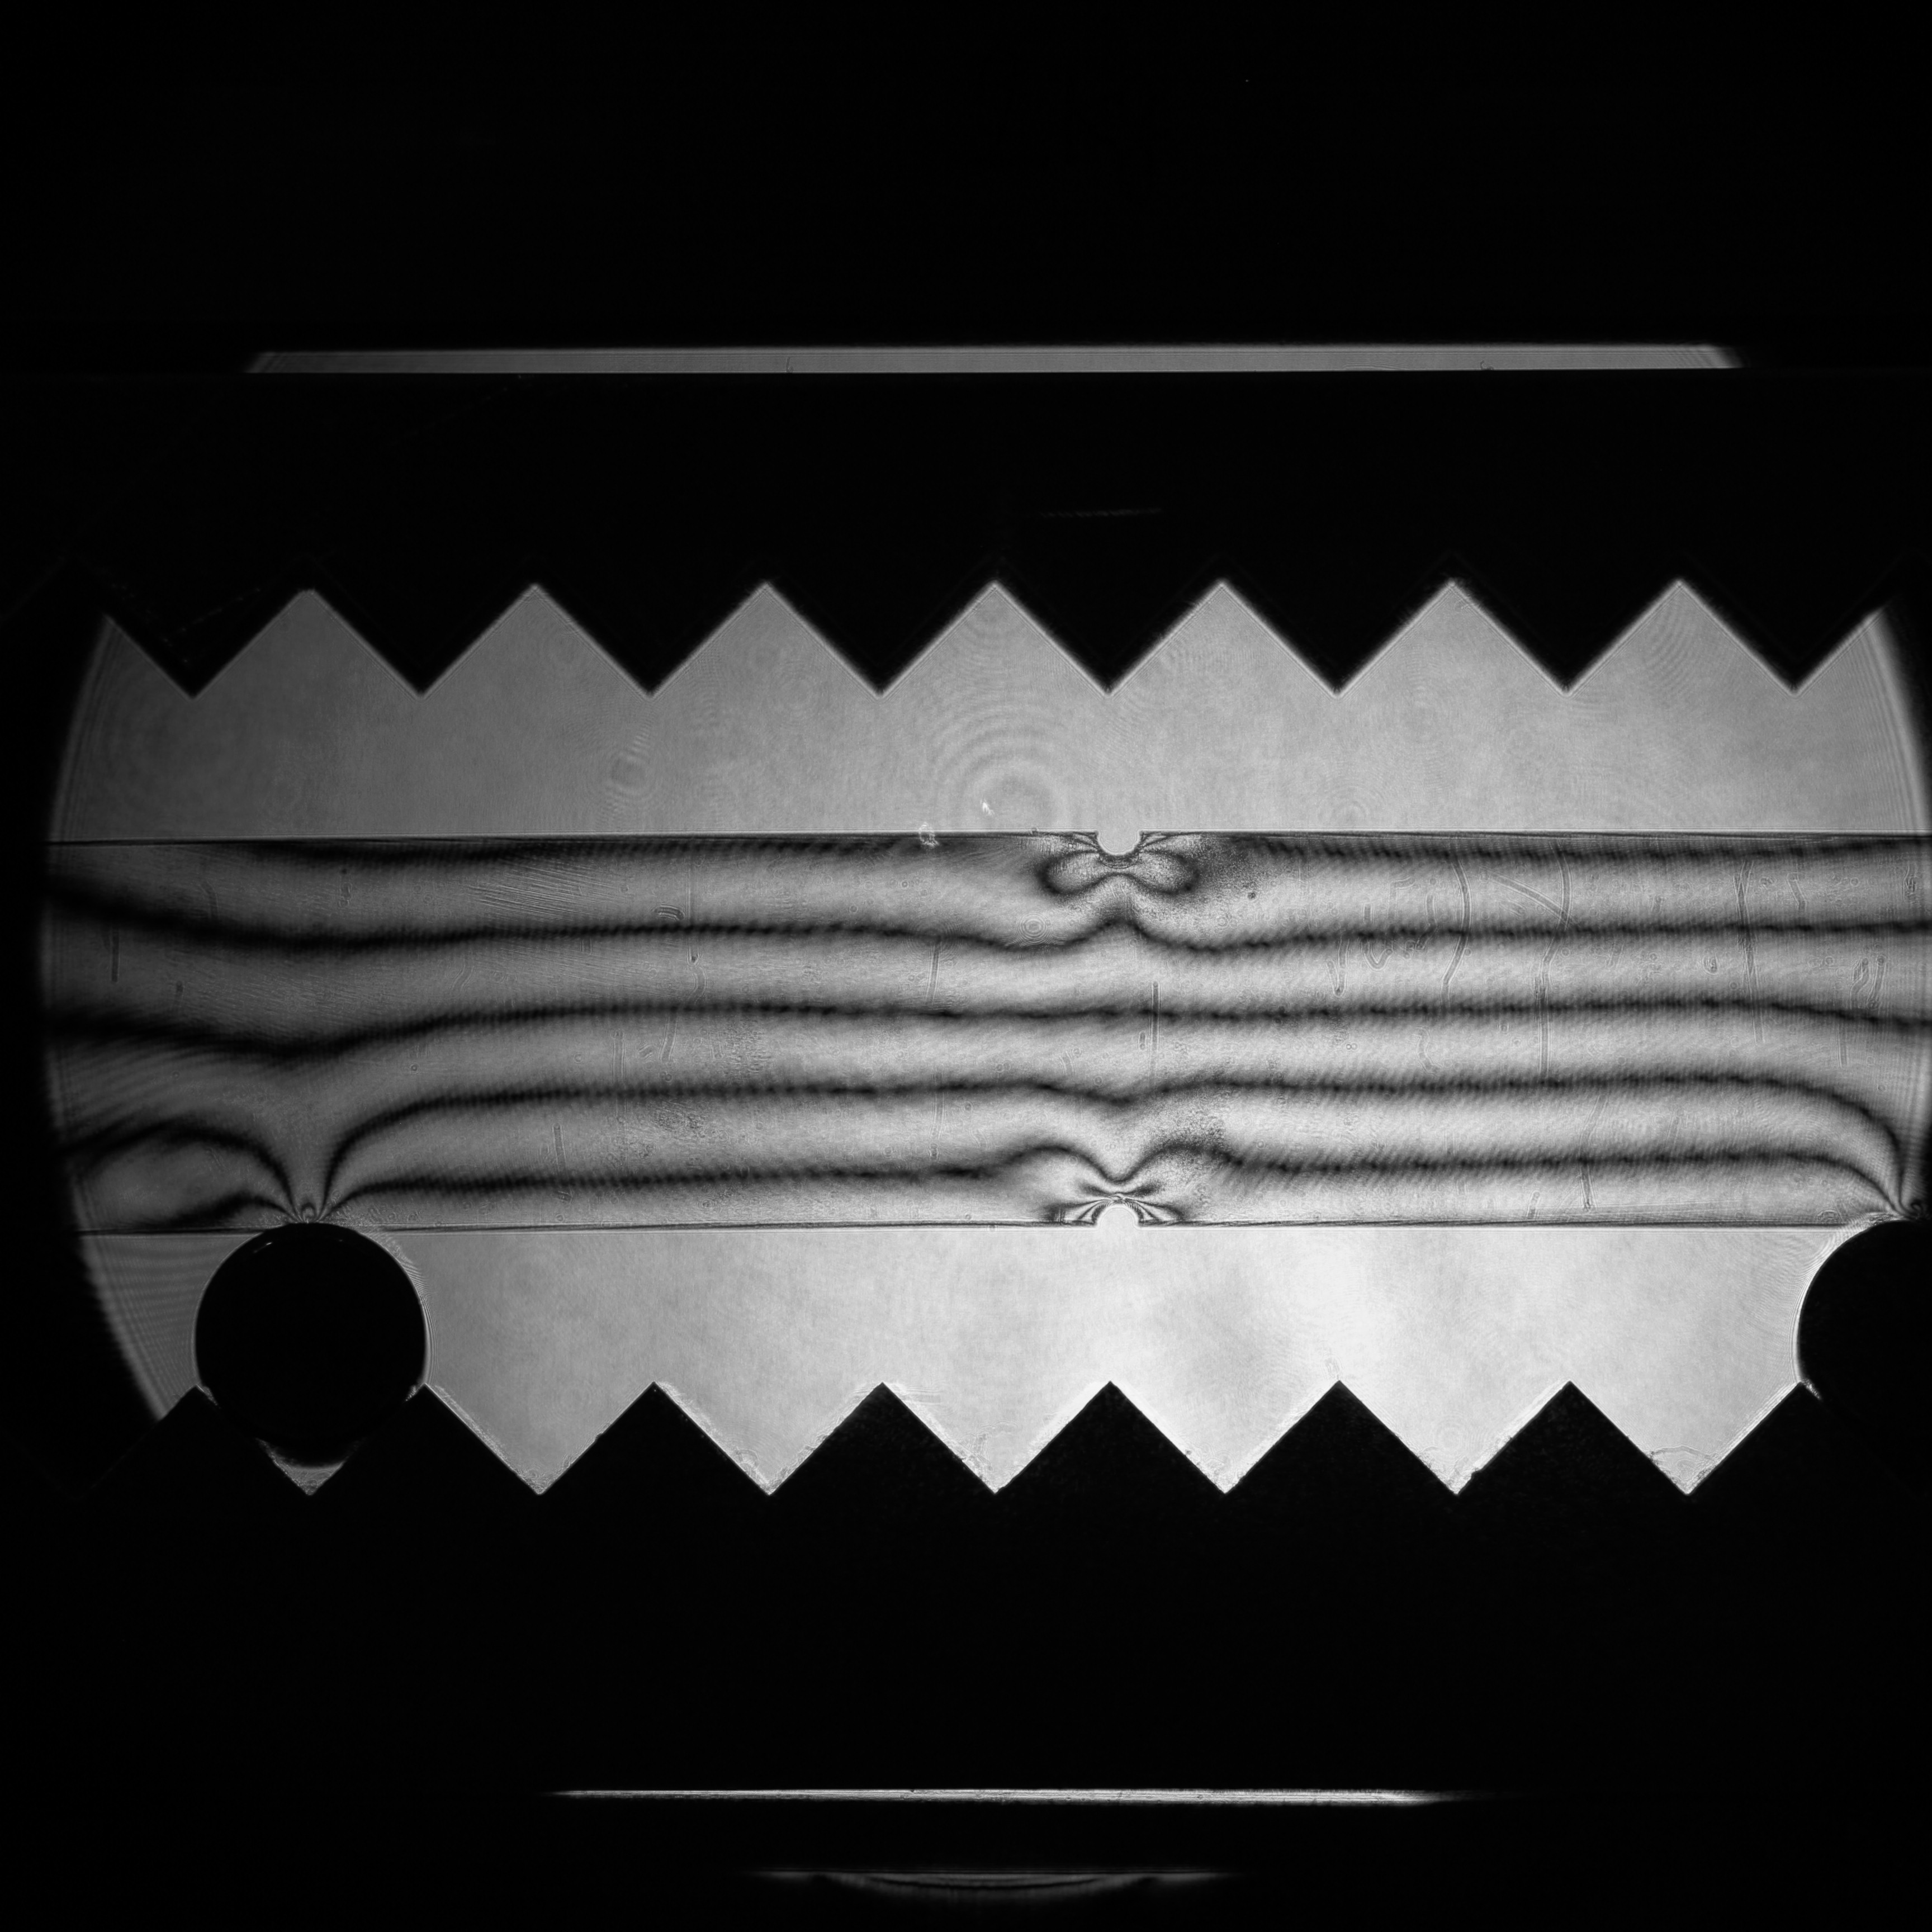
\includegraphics[width=\textwidth]{ρ=1.jpg}
        \caption{実験による光弾性画像 ($\rho=1$)}
    \end{minipage}
    \hfill
    \begin{minipage}[b]{0.48\textwidth}
        \centering
        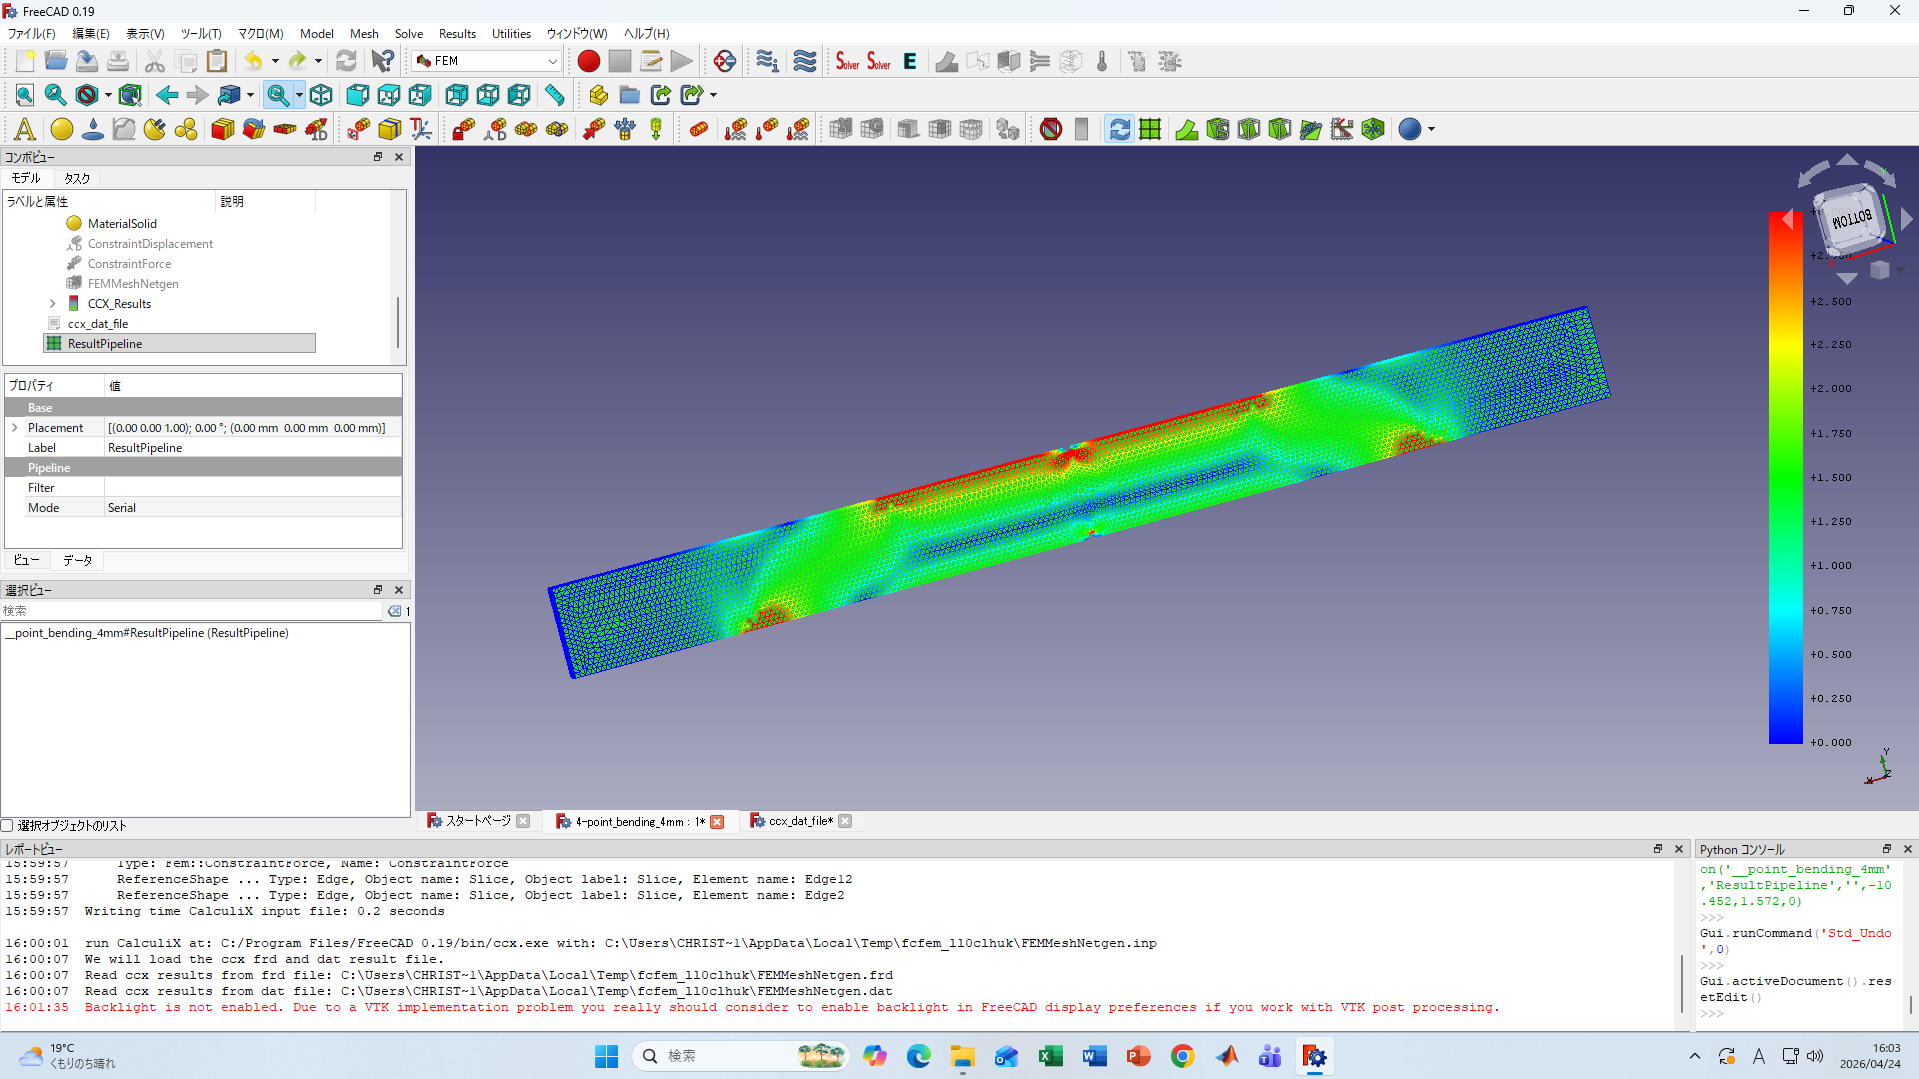
\includegraphics[width=\textwidth]{メッシュ_1mm.png}
        \caption{有限要素法による応力分布 ($\rho=1$)}
    \end{minipage}
\end{figure}

この2つの画像を比較すると、どちらも切り欠きの部分において最大の応力が加わっていることが定性的に一致していることが分かる。\\
一方で、課題2の光弾性画像においては主応力差に起因する縞次数のみが等高線状に観測されるのに対し、有限要素法のシミュレーションにおいては応力分布を連続なグラデーションとして観測できるという違いがある。\\
また、課題2の光弾性実験が現実の治具との接触や摩擦などの物理的条件をすべて含んだ結果であるのに対し、有限要素法はメッシュサイズの粗密による影響（メッシュ依存性）を強く受ける。これらのことを考慮すると、現実の現象として発生している応力場は、実際の光弾性画像においてより忠実に表されているといえる。


\section{総括}
本実験を通して、光弾性法を用いた応力場の評価手法、および超音波計測による弾性係数の評価手法について...
% TODO: レポート全体のまとめを記述する

% --------------------------------------------------
% 参考文献
% --------------------------------------------------
\section*{参考文献}
\begin{enumerate}[label={[\arabic*]}]
    \item 著者名, 『書籍名』, 出版社, 発行年.
    \item 物理工学科 実験指導書, 2026.
\end{enumerate}

\end{document}